% Options for packages loaded elsewhere
\PassOptionsToPackage{unicode}{hyperref}
\PassOptionsToPackage{hyphens}{url}
\PassOptionsToPackage{dvipsnames,svgnames,x11names}{xcolor}
%
\documentclass[
  11pt,
]{article}

\usepackage{amsmath,amssymb}
\usepackage{iftex}
\ifPDFTeX
  \usepackage[T1]{fontenc}
  \usepackage[utf8]{inputenc}
  \usepackage{textcomp} % provide euro and other symbols
\else % if luatex or xetex
  \usepackage{unicode-math}
  \defaultfontfeatures{Scale=MatchLowercase}
  \defaultfontfeatures[\rmfamily]{Ligatures=TeX,Scale=1}
\fi
\usepackage{lmodern}
\ifPDFTeX\else  
    % xetex/luatex font selection
    \setmainfont[]{Aptos}
\fi
% Use upquote if available, for straight quotes in verbatim environments
\IfFileExists{upquote.sty}{\usepackage{upquote}}{}
\IfFileExists{microtype.sty}{% use microtype if available
  \usepackage[]{microtype}
  \UseMicrotypeSet[protrusion]{basicmath} % disable protrusion for tt fonts
}{}
\makeatletter
\@ifundefined{KOMAClassName}{% if non-KOMA class
  \IfFileExists{parskip.sty}{%
    \usepackage{parskip}
  }{% else
    \setlength{\parindent}{0pt}
    \setlength{\parskip}{6pt plus 2pt minus 1pt}}
}{% if KOMA class
  \KOMAoptions{parskip=half}}
\makeatother
\usepackage{xcolor}
\setlength{\emergencystretch}{3em} % prevent overfull lines
\setcounter{secnumdepth}{-\maxdimen} % remove section numbering
% Make \paragraph and \subparagraph free-standing
\makeatletter
\ifx\paragraph\undefined\else
  \let\oldparagraph\paragraph
  \renewcommand{\paragraph}{
    \@ifstar
      \xxxParagraphStar
      \xxxParagraphNoStar
  }
  \newcommand{\xxxParagraphStar}[1]{\oldparagraph*{#1}\mbox{}}
  \newcommand{\xxxParagraphNoStar}[1]{\oldparagraph{#1}\mbox{}}
\fi
\ifx\subparagraph\undefined\else
  \let\oldsubparagraph\subparagraph
  \renewcommand{\subparagraph}{
    \@ifstar
      \xxxSubParagraphStar
      \xxxSubParagraphNoStar
  }
  \newcommand{\xxxSubParagraphStar}[1]{\oldsubparagraph*{#1}\mbox{}}
  \newcommand{\xxxSubParagraphNoStar}[1]{\oldsubparagraph{#1}\mbox{}}
\fi
\makeatother


\providecommand{\tightlist}{%
  \setlength{\itemsep}{0pt}\setlength{\parskip}{0pt}}\usepackage{longtable,booktabs,array}
\usepackage{calc} % for calculating minipage widths
% Correct order of tables after \paragraph or \subparagraph
\usepackage{etoolbox}
\makeatletter
\patchcmd\longtable{\par}{\if@noskipsec\mbox{}\fi\par}{}{}
\makeatother
% Allow footnotes in longtable head/foot
\IfFileExists{footnotehyper.sty}{\usepackage{footnotehyper}}{\usepackage{footnote}}
\makesavenoteenv{longtable}
\usepackage{graphicx}
\makeatletter
\def\maxwidth{\ifdim\Gin@nat@width>\linewidth\linewidth\else\Gin@nat@width\fi}
\def\maxheight{\ifdim\Gin@nat@height>\textheight\textheight\else\Gin@nat@height\fi}
\makeatother
% Scale images if necessary, so that they will not overflow the page
% margins by default, and it is still possible to overwrite the defaults
% using explicit options in \includegraphics[width, height, ...]{}
\setkeys{Gin}{width=\maxwidth,height=\maxheight,keepaspectratio}
% Set default figure placement to htbp
\makeatletter
\def\fps@figure{htbp}
\makeatother

\usepackage{booktabs}
\usepackage{longtable}
\usepackage{array}
\usepackage{multirow}
\usepackage{wrapfig}
\usepackage{float}
\usepackage{colortbl}
\usepackage{pdflscape}
\usepackage{tabu}
\usepackage{threeparttable}
\usepackage{threeparttablex}
\usepackage[normalem]{ulem}
\usepackage{makecell}
\usepackage{xcolor}
\usepackage{pdfpages}
\usepackage{fontspec}
\usepackage[bottom]{footmisc}
\setmainfont{Aptos}[Path="C:/Users/ginow/AppData/Roaming/TinyTeX/texmf-dist/fonts/truetype/aptos/", Extension=".ttf"]
\usepackage{fancyhdr}
\pagestyle{fancy}
\fancyhf{}
\cfoot{\thepage}
\setlength{\footskip}{10pt}
\setlength{\skip\footins}{15pt}
\renewcommand{\footrulewidth}{0pt}
\floatplacement{figure}{H}
\floatplacement{table}{H}
\usepackage{geometry}
\geometry{ left=3cm, right=3cm, top=2.5cm, bottom=2.5cm }
\usepackage{placeins}
\usepackage{ragged2e}
\usepackage{float}
\usepackage{setspace}
\renewcommand{\familydefault}{\sfdefault}
\AtBeginDocument{\renewcommand{\baselinestretch}{1.5}\justifying}
\usepackage{xcolor}
\definecolor{mybgcolor}{HTML}{01376B}
\usepackage{pagecolor}
\makeatletter
\@ifpackageloaded{caption}{}{\usepackage{caption}}
\AtBeginDocument{%
\ifdefined\contentsname
  \renewcommand*\contentsname{Tabla de contenidos}
\else
  \newcommand\contentsname{Tabla de contenidos}
\fi
\ifdefined\listfigurename
  \renewcommand*\listfigurename{Listado de Figuras}
\else
  \newcommand\listfigurename{Listado de Figuras}
\fi
\ifdefined\listtablename
  \renewcommand*\listtablename{Listado de Tablas}
\else
  \newcommand\listtablename{Listado de Tablas}
\fi
\ifdefined\figurename
  \renewcommand*\figurename{Figura}
\else
  \newcommand\figurename{Figura}
\fi
\ifdefined\tablename
  \renewcommand*\tablename{Tabla}
\else
  \newcommand\tablename{Tabla}
\fi
}
\@ifpackageloaded{float}{}{\usepackage{float}}
\floatstyle{ruled}
\@ifundefined{c@chapter}{\newfloat{codelisting}{h}{lop}}{\newfloat{codelisting}{h}{lop}[chapter]}
\floatname{codelisting}{Listado}
\newcommand*\listoflistings{\listof{codelisting}{Listado de Listados}}
\makeatother
\makeatletter
\makeatother
\makeatletter
\@ifpackageloaded{caption}{}{\usepackage{caption}}
\@ifpackageloaded{subcaption}{}{\usepackage{subcaption}}
\makeatother

\ifLuaTeX
\usepackage[bidi=basic]{babel}
\else
\usepackage[bidi=default]{babel}
\fi
\babelprovide[main,import]{spanish}
\ifPDFTeX
\else
\babelfont{rm}[]{Aptos}
\fi
% get rid of language-specific shorthands (see #6817):
\let\LanguageShortHands\languageshorthands
\def\languageshorthands#1{}
\ifLuaTeX
  \usepackage{selnolig}  % disable illegal ligatures
\fi
\usepackage{bookmark}

\IfFileExists{xurl.sty}{\usepackage{xurl}}{} % add URL line breaks if available
\urlstyle{same} % disable monospaced font for URLs
\hypersetup{
  pdflang={es},
  colorlinks=true,
  linkcolor={blue},
  filecolor={Maroon},
  citecolor={Blue},
  urlcolor={Blue},
  pdfcreator={LaTeX via pandoc}}


\author{}
\date{}

\begin{document}

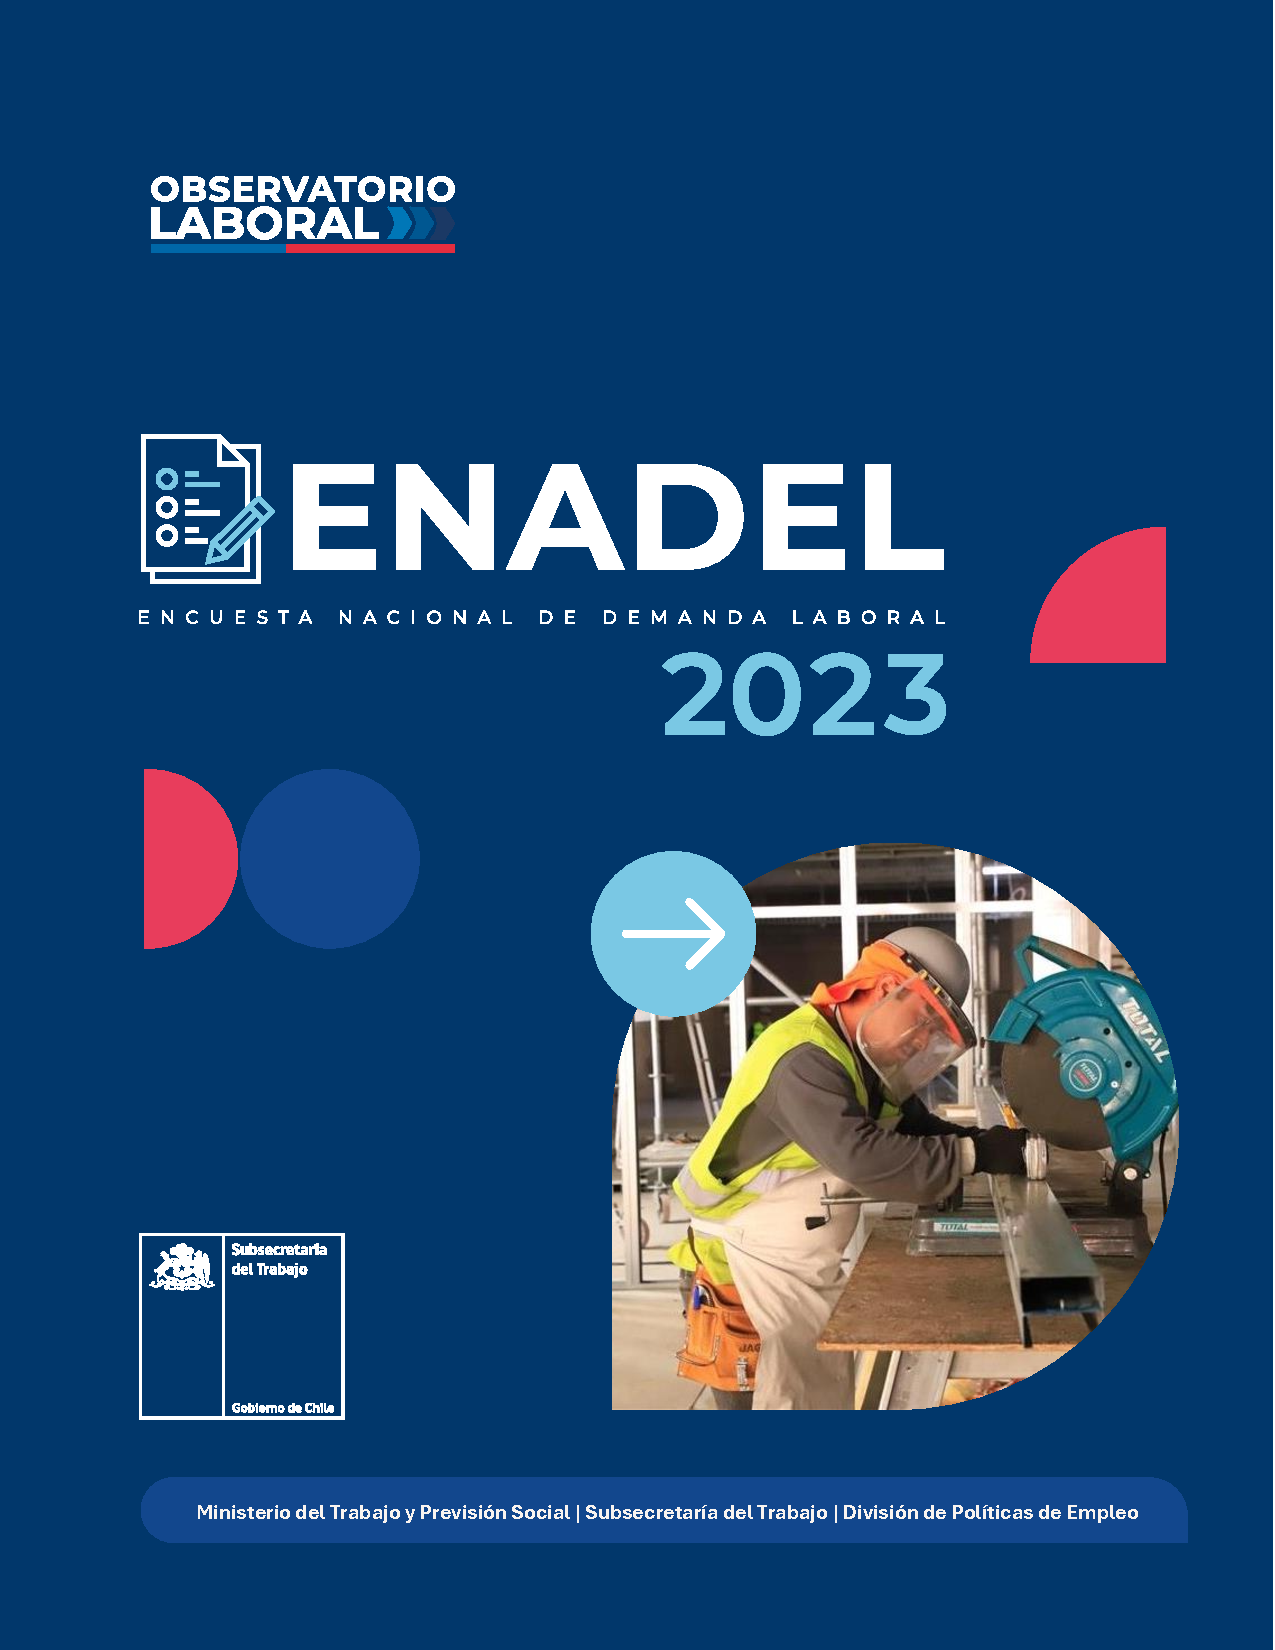
\includepdf[pages=-]{../Quarto/Portada/Portadas-Enadel-2023-1.pdf}


\newpage

\pagecolor{mybgcolor} 
\color{white}

\centering


\includegraphics[width=0.5\textwidth]{../Logotipo ENADEL/Logotipo ENADEL 2023.png}
\vspace{2cm}

\noindent Ministerio del Trabajo y Previsión Social

División de Políticas de Empleo\textbackslash{} Subsecretaría del
Trabajo

\justifying

El presente documento analiza los resultados de la Encuesta Nacional de
Demanda Laboral (ENADEL) 2023, que busca identificar y caracterizar el
capital humano requerido por las empresas de los distintos sectores
productivos del país, generando información sobre la demanda actual de
ocupaciones de las empresas, detectando requisitos y problemas de
contratación. Al igual que versiones anteriores de esta encuesta, se
puso el foco en dos sectores de actividad económica: Construcción y el
sector Agrícola.

\newpage

\pagecolor{white} \% Volver al fondo blanco para el resto del documento
\color{black}

\newpage
\renewcommand{\contentsname}{Índice} 
\tableofcontents

\newpage

\subsection{Descripción General: Empresas y
Trabajadores}\label{descripciuxf3n-general-empresas-y-trabajadores}

La muestra de ENADEL 2023 encuesta a 5.820 empresas que suman 485.256
trabajadores (a nivel muestral). Estas representan a 82.052 empresas y
5.611.196 trabajadores a nivel nacional. La Tabla~\ref{tbl-region}
muestra la distribución en las distintas regiones del país, dónde un
\text{53,6}\% de las empresas y un \text{65,6}\% de los trabajadores se
encuentran en la región Metropolitana.

\vspace{5mm}

\FloatBarrier

\begin{table}

\caption{\label{tbl-region}Resultados de la encuesta}

\centering{

\centering
\begin{tabular}{lll}
\toprule
Región & \% Empresas & \% Trabajadores\\
\midrule
Arica y Parinacota & 0,67\% & 0,33\%\\
Tarapacá & 1,69\% & 1,07\%\\
Antofagasta & 2,6\% & 1,82\%\\
Atacama & 0,76\% & 0,54\%\\
Coquimbo & 2,78\% & 1,86\%\\
\addlinespace
Valparaíso & 9,05\% & 6,5\%\\
Metropolitana & 53,61\% & 65,59\%\\
O'Higgins & 5,1\% & 4,21\%\\
Maule & 1,54\% & 1,01\%\\
Ñuble & 6,66\% & 4,96\%\\
\addlinespace
Biobío & 1,35\% & 0,69\%\\
Araucanía & 4,59\% & 3,45\%\\
Los Ríos & 0,39\% & 0,25\%\\
Los Lagos & 0,98\% & 0,64\%\\
Aysén & 4,92\% & 4,74\%\\
\addlinespace
Magallanes & 3,3\% & 2,34\%\\
\bottomrule
\multicolumn{3}{l}{\rule{0pt}{1em}Fuente: Elaboración propia utilizando datos de ENADEL 2023, datos expandidos.}\\
\end{tabular}

}

\end{table}%

\FloatBarrier

La Figura~\ref{fig-combined} muestra el porcentaje de empresas y
trabajadores según tamaño de empresas, utilizando la clasificación por
número de trabajadores, cómo por volumen de venta. Con respecto a la
primera clasificación, el 74,6\% de las empresas tiene menos de 50
trabajadores --acumulando un 23,8\% del total-- y casi el 50\% de los
trabajadores están en empresas grandes --que corresponden a un 6,5\% del
total. Si se analiza según tamaño de ventas, más de la mitad de las
empresas tienen un volumen de venta de entre 2.400 y 24.999 UF
(``Pequeñas'') y más de un cuarto venden entre 25.000 y 100.000 UF al
año (``Mediana''). Sin embargo, casi un tercio de los trabajadores están
en empresas grandes (más de 100.000 UF).

\FloatBarrier

\begin{figure}[H]

\caption{\label{fig-combined}Gráfico combinado de resultados}

\centering{

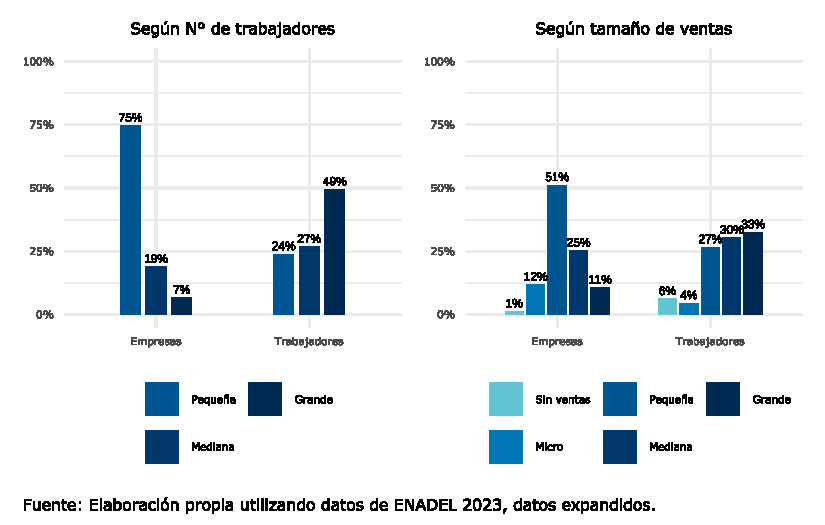
\includegraphics[width=1\textwidth,height=\textheight]{Reporte_files/figure-pdf/fig-combined-1.pdf}

}

\end{figure}%

\FloatBarrier

Al revisar la distribución por sector de actividad económica
Tabla~\ref{tbl-acteco} se tiene que una de cada cinco empresas pertenece
al sector de Comercio, seguido por el sector Construcción
(\text{15,5}\%) y el sector de Industrias Manufactureras (11,4\%). Con
respecto al volumen de trabajadores, el sector Comercio también lidera
(17,8\%) seguido por el sector Construcción (14,4\%) y el sector de
Servicios Administrativos y de Apoyo que, siendo sector intensivo en
trabajo, un 9,1\% de las empresas acumula el 13,5\% de trabajadores y
trabajadoras.

\FloatBarrier

\begin{table}

\caption{\label{tbl-acteco}Empresas y trabajadores según sector de
actividad económica}

\centering{

\centering
\begin{tabular}{>{\raggedright\arraybackslash}p{11cm}ll}
\toprule
Actividad Económica & \% Empresas & \% Trabajadores\\
\midrule
Comercio & 20,6\% & 17,78\%\\
Construcción & 15,54\% & 14,42\%\\
Servicios administrativos y de apoyo & 9,08\% & 13,5\%\\
Industria manufacturera & 11,39\% & 11,81\%\\
Actividades profesionales & 10,82\% & 10,97\%\\
\addlinespace
Silvoagropecuario & 8,64\% & 8,33\%\\
Transporte y almacenamiento & 7,62\% & 5,91\%\\
Administración pública & 0,69\% & 5,46\%\\
Alojamiento y de servicio de comidas & 6,79\% & 4,03\%\\
Información y comunicaciones & 3,02\% & 2,61\%\\
\addlinespace
Actividades inmobiliarias & 3,15\% & 2,6\%\\
Actividades financieras y de seguros & 1,88\% & 1,69\%\\
Pesca y acuicultura & 0,77\% & 0,9\%\\
\bottomrule
\multicolumn{3}{l}{\rule{0pt}{1em}Fuente: Elaboración propia utilizando datos de ENADEL 2023, datos expandidos.}\\
\end{tabular}

}

\end{table}%

\FloatBarrier

\subsubsection{Contratados en los últimos 12
meses}\label{contratados-en-los-uxfaltimos-12-meses}

El 87,1\% de las empresas declaró que sí contrató personas nuevas
durante los últimos 12 meses, mientras que el 12,9\% declara que no
contrató personas nuevas durante el mismo período. La
Tabla~\ref{tbl-contratos_totales} muestra la proporción de empresas,
según sector de actividad económica, que tuvieron contrataciones nuevas
durante los últimos 12 meses. El 98.9\% de las empresas del sector de
pesca y acuicultura respondieron afirmativamente, mientras que el sector
con menor proporción fue el de Actividades Inmobiliarias, dónde el
24,9\% de firmas no tuvieron contrataciones durante los últimos 12
meses.

\FloatBarrier

\begin{table}

\caption{\label{tbl-contratos_totales}Porcentaje de empresas que
contrataron en los últimos 12 meses por sector económico}

\centering{

\centering
\begin{tabular}{>{\raggedright\arraybackslash}p{11cm}ll}
\toprule
Actividad Económica & \% Si & \% No\\
\midrule
Actividades profesionales & 90,4\% & 9,6\%\\
Actividades financieras y de seguros & 83,9\% & 16,1\%\\
Actividades inmobiliarias & 75,1\% & 24,9\%\\
Administración pública & 90,3\% & 9,7\%\\
Alojamiento y de servicio de comidas & 92,9\% & 7,1\%\\
\addlinespace
Comercio & 84,8\% & 15,2\%\\
Construcción & 89,3\% & 10,7\%\\
Industria manufacturera & 87,3\% & 12,7\%\\
Información y comunicaciones & 90,3\% & 9,7\%\\
Servicios administrativos y de apoyo & 87,5\% & 12,5\%\\
\addlinespace
Silvoagropecuario & 83,6\% & 16,4\%\\
Pesca y acuicultura & 98,9\% & 1,1\%\\
Transporte y almacenamiento & 85\% & 15\%\\
Total & 87,6\% & 12,4\%\\
\bottomrule
\multicolumn{3}{l}{\rule{0pt}{1em}Fuente: Elaboración propia utilizando datos de ENADEL 2023, datos expandidos.}\\
\end{tabular}

}

\end{table}%

\FloatBarrier

\subparagraph{Contrataciones por
ocupación}\label{contrataciones-por-ocupaciuxf3n}

Se contrataron cargos\footnote{Contrataciones señaladas para los módulos
  de ``Directores y gerentes'', ``Jefatura/ADP'', ``Ocupaciones
  Elementales'' y ``Otros Cargos''.} nuevos en 354 ocupaciones
(representando a 1.206.992 contrataciones totales en los últimos 12
meses, cv = 6,8\%), sin embargo, la Tabla~\ref{tbl-contratados_u12} sólo
muestra aquellas para las cuáles el coeficiente de variación es menor a
20\%\footnote{La convención es considerar cómo robustas estimaciones con
  un cv menor al 15\%. Dado que estas son pocas, se presentan todas las
  ocupaciones con un cv menor a 20\%.}. Las ocupaciones con más
contratos en los últimos 12 meses fueron ``Obreros de explotaciones
agrícolas'', ``Auxiliares de aseo de oficinas, hoteles y otros
establecimientos'' y ``Vendedores y asistentes de venta de tiendas,
almacenes y puestos de mercado''.

\begin{table}

\caption{\label{tbl-contratados_u12}Contratados últimos 12 meses, por
ocupación.}

\centering{

\centering
\begin{tabular}{>{\raggedleft\arraybackslash}p{1.2cm}>{\raggedright\arraybackslash}p{11cm}rl}
\toprule
CIUO\_08 & Glosa & Contratados & cv\\
\midrule
9211 & Obreros de explotaciones agrícolas & 300480 & 19,2\%\\
9112 & Auxiliares de aseo de oficinas, hoteles y otros establecimientos & 71821 & 16,4\%\\
5223 & Vendedores y asistentes de venta de tiendas, almacenes y puestos de mercado & 23492 & 15,7\%\\
5414 & Guardias de seguridad & 17719 & 12,9\%\\
5131 & Garzones de mesa & 13484 & 10,4\%\\
\addlinespace
8332 & Conductores de camiones pesados y de alto tonelaje & 12410 & 9,5\%\\
5120 & Cocineros & 7623 & 14,7\%\\
3123 & Supervisores de la construcción & 5224 & 19,2\%\\
2243 & Ingenieros en prevención de riesgos y otros profesionales de la seguridad e higiene laboral y ambiental & 2971 & 19,2\%\\
8331 & Conductores de buses y trolebuses & 2968 & 16,6\%\\
\addlinespace
8350 & Tripulantes de cubierta de barco & 1639 & 18,7\%\\
\bottomrule
\multicolumn{4}{l}{\rule{0pt}{1em}Fuente: Elaboración propia utilizando datos de ENADEL 2023, datos expandidos.}\\
\end{tabular}

}

\end{table}%

\newpage

\subparagraph{Contrataciones por ocupación: Sector
Construcción}\label{contrataciones-por-ocupaciuxf3n-sector-construcciuxf3n}

En el módulo del sector Construcción se consulta sobre las
contrataciones de 25 cargos específicos, con un total de 365.712
contrataciones en los últimos 12 meses (cv=29,2\%). La
Tabla~\ref{tbl-contratados_u12_constru} muestra la proporción de
contratados por cargo, con respecto al total de este módulo. El cargo de
``Obreros y jornales'' es el que concentra la mayor cantidad de
contrataciones, seguido por ``Carpinteros'' y por ``Electricistas
(técnicos y/o maestros)''.

\begin{table}

\caption{\label{tbl-contratados_u12_constru}Proporción de contrataciones
por ocupación, sector construcción.}

\centering{

\centering
\begin{tabular}{>{\raggedright\arraybackslash}p{12cm}l}
\toprule
Cargo Construcción & \%\\
\midrule
Obreros y jornales & 23,2\%\\
Carpinteros & 12,2\%\\
Electricistas (técnicos y/o maestros) & 11,5\%\\
Otros maestros de primera y segunda & 9,7\%\\
Albañiles & 7\%\\
\addlinespace
Enfierradores & 4\%\\
Concreteros & 3,7\%\\
Operadores de maquinaria pesada & 3,2\%\\
Pintores & 3,1\%\\
Operadores de maquinaria liviana & 3\%\\
\addlinespace
Ingenieros, prevencionistas, arqueólogos, otros profesionales & 2,6\%\\
Baldoseros y ceramistas & 2,6\%\\
Soldadores & 2,4\%\\
Capataces & 2,3\%\\
Encargados de Obra & 2,1\%\\
\addlinespace
Electrónicos, electromecánicos e instrumentistas & 2,1\%\\
Mecánicos & 1,6\%\\
Trazadores & 1,1\%\\
Bodegueros y cardcheckers & 1\%\\
Sanitarios y gásfiteres & 0,4\%\\
\addlinespace
Instaladores de gas & 0,4\%\\
Operadores planta asfalto y áridos & 0,3\%\\
Laboratoristas & 0,2\%\\
Tuberos y peradores de termofusión & 0,2\%\\
Buzos & 0\%\\
\bottomrule
\multicolumn{2}{l}{\rule{0pt}{1em}Fuente: Elaboración propia utilizando datos de ENADEL 2023, datos expandidos.}\\
\end{tabular}

}

\end{table}%

\subparagraph{Contrataciones por ocupación: Sector
Agrícola}\label{contrataciones-por-ocupaciuxf3n-sector-agruxedcola}

En el módulo del sector Agrícola se consulta sobre las contrataciones de
15 cargos específicos, con un total de 321.395 contrataciones en los
últimos 12 meses (cv=21,6\%), cuya distribución en los distintos cargos
se muestra en la Tabla~\ref{tbl-contratados_u12_agricola}. Las
ocupaciones de ``Obrero agrícola de cosecha'' y ``Obrero agrícola de
packing frutícola, bodega, estabilización, embotellado'' son las que
lideran las contrataciones durante los últimos 12 meses.

\begin{table}

\caption{\label{tbl-contratados_u12_agricola}Proporción de
contrataciones por ocupación, sector agrícola}

\centering{

\centering
\begin{tabular}{ll}
\toprule
Cargo Agrícola & \%\\
\midrule
Obrero agrícola de cosecha & 37,6\%\\
Obrero agrícola de packing frutícola, bodega, estabilización, embotellado & 37,4\%\\
Obrero agrícola de poda, raleo & 11,3\%\\
Obrero agrícola de siembra, viveros & 3,7\%\\
Obrero agrícola de riego, aplicación de agroquímicos & 3,2\%\\
\addlinespace
Obrero forestal de cosecha & 1,9\%\\
Obrero agrícola de almácigos & 1,7\%\\
Obrero forestal de siembra & 1,2\%\\
Obrero pecuario de crianza, alimentación, pastoreo & 0,8\%\\
Obrero agroindustrial gestión de cría y engorda & 0,6\%\\
\addlinespace
Obrero forestal en labores de aserrador & 0,3\%\\
Obrero pecuario de ordeña & 0,2\%\\
Obrero agrícola de manejo reproductivo y sanitario & 0\%\\
Obrero agroindustrial en matadero & 0\%\\
Obrero agroindustrial limpieza, control plagas y enfermedades & 0\%\\
\bottomrule
\multicolumn{2}{l}{\rule{0pt}{1em}Fuente: Elaboración propia utilizando datos de ENADEL 2023, datos expandidos.}\\
\end{tabular}

}

\end{table}%

\subsubsection{Vacantes en los últimos 12
meses}\label{vacantes-en-los-uxfaltimos-12-meses}

El 72,05\% de las empresas declaró que sí tuvo vacantes no llenadas
durante los últimos 12 meses, mientras que el 27,95\% declara que no
tuvo vacantes no llenadas durante el mismo período.

La Tabla~\ref{tbl-vacantes_totales_sector} muestra la proporción de
empresas, según sector de actividad económica, que tuvieron vacantes no
llenadas durante los últimos 12 meses. El 89.5\% de las empresas del
sector de ``Información y comunicaciones'' tuvieron vacantes no
llenadas, lo mismo ocurre con el 87.7\% de las personas jurídicas del
sector de ``Administración pública'' y el 80.2\% del sector de
``Actividades profesionales''. Por otro lado, el sector de actividad
económica con un menor porcentaje de empresas que tuvieron vacantes no
llenadas fue el ``Silvoagropecuario''.

\begin{table}

\caption{\label{tbl-vacantes_totales_sector}Porcentaje de empresas con
vacantes no cubiertas}

\centering{

\centering
\begin{tabular}{>{\raggedright\arraybackslash}p{10cm}ll}
\toprule
Sector Actividad Económica & \% Sí & \% No\\
\midrule
Información y comunicaciones & 89,5\% & 10,5\%\\
Administración pública & 87,7\% & 12,3\%\\
Actividades profesionales & 80,2\% & 19,8\%\\
Alojamiento y de servicio de comidas & 78,3\% & 21,7\%\\
Transporte y almacenamiento & 78,3\% & 21,7\%\\
\addlinespace
Servicios administrativos y de apoyo & 76,4\% & 23,6\%\\
Industria manufacturera & 73,7\% & 26,3\%\\
Comercio & 72,3\% & 27,7\%\\
Construcción & 67,8\% & 32,2\%\\
Actividades financieras y de seguros & 67,6\% & 32,4\%\\
\addlinespace
Actividades inmobiliarias & 63\% & 37\%\\
Pesca y acuicultura & 61,7\% & 38,3\%\\
Silvoagropecuario & 49,4\% & 50,6\%\\
\bottomrule
\multicolumn{3}{l}{\rule{0pt}{1em}Fuente: Elaboración propia utilizando datos de ENADEL 2023, datos expandidos.}\\
\end{tabular}

}

\end{table}%

Durante el resto de esta sección se hará referencia a las ocupaciones
que tengan vacantes sin llenar durante los últimos 12 meses como
\textbf{ocupaciones de difícil cobertura}.

\newpage

\subparagraph{Ocupaciones de difícil
cobertura}\label{ocupaciones-de-difuxedcil-cobertura}

Se declararon vacantes\footnote{Vacantes señaladas para los módulos de
  ``Directores y gerentes'', ``Jefatura/ADP'', ``Ocupaciones
  Elementales'' y ``Otros Cargos''.} sin llenar en 215 ocupaciones
(68.365 vacantes, cv=12,3\%), sin embargo, la
Tabla~\ref{tbl-vacantes_tot} sólo muestra aquellas para las cuáles el
coeficiente de variación es menor a 40\%\footnote{La convención es
  considerar cómo robustas estimaciones con un cv menor al 15\%. Dado
  que esto no se cumple, se presentan todas las ocupaciones con un cv
  menor a 40\%.}. La tabla completa con todas las ocupaciones de difícil
cobertura se puede encontrar en el \textbf{Apéndice A: Ocupaciones de
Difícil Cobertura}.

\begin{table}

\caption{\label{tbl-vacantes_tot}Ocupaciones de difícil cobertura,
ENADEL 2023.}

\centering{

\centering
\begin{tabular}{>{\raggedleft\arraybackslash}p{1.2cm}>{\raggedright\arraybackslash}p{11cm}rl}
\toprule
CIUO 08 & Glosa & Vacantes & cv\\
\midrule
9211 & Obreros de explotaciones agrícolas & 14374 & 38,3\%\\
5414 & Guardias de seguridad & 1193 & 39,4\%\\
9112 & Auxiliares de aseo de oficinas, hoteles y otros establecimientos & 1022 & 36,6\%\\
5223 & Vendedores y asistentes de venta de tiendas, almacenes y puestos de mercado & 476 & 35,2\%\\
5120 & Cocineros & 337 & 38,6\%\\
\addlinespace
8332 & Conductores de camiones pesados y de alto tonelaje & 232 & 33,8\%\\
\bottomrule
\multicolumn{4}{l}{\rule{0pt}{1em}Fuente: Elaboración propia utilizando datos de ENADEL 2023, datos expandidos.}\\
\end{tabular}

}

\end{table}%

La ocupación más demandadas que tiene difícil cobertura es ``Obreros de
explotaciones agrícolas'', con más de 14 mil vacantes; seguido de lejos
por ``Guardias de seguridad'', ``Auxiliares de aseo de oficinas, hoteles
y otros establecimientos'' y ``Vendedores y asistentes de venta de
tiendas, almacenes y puestos de mercado'', con 1193, 1022 y 476
vacantes, respectivamente.

La Tabla~\ref{tbl-vacantes_region} muestra la ocupación de difícil
cobertura con mayor cantidad de vacantes por región dónde, si bien se
confirma la prevalencia de ``Obreros de explotaciones agrícolas'' en 7
regiones, también saltan a la vista otros patrones como la demanda del
rubro de la construcción hacia el norte y de la industria manufacturera
en el Maule y la Araucanía.

\begin{table}

\caption{\label{tbl-vacantes_region}Ocupación de difícil cobertura con
mayor cantidad de vacantes, por región.}

\centering{

\centering
\begin{tabular}{l>{\raggedright\arraybackslash}p{7cm}rr}
\toprule
Región & Ocupación & CIUO 08 & Vacantes\\
\midrule
Arica y Parinacota & Obreros de la construcción de edificios & 9313 & 91\\
Tarapacá & Otros operarios de la construcción (obra gruesa) no clasificados previamente & 7119 & 112\\
Antofagasta & Soldadores y oxicortadores & 7212 & 66\\
Atacama & Obreros de explotaciones agrícolas & 9211 & 2943\\
Coquimbo & Cocineros de comida rápida & 9411 & 236\\
\addlinespace
Valparaíso & Obreros de explotaciones agrícolas & 9211 & 1076\\
Metropolitana & Obreros de explotaciones agrícolas & 9211 & 3376\\
O'Higgins & Secretarios generales & 4120 & 269\\
Maule & Obreros de la industria manufacturera no clasificados previamente & 9329 & 93\\
Ñuble & Agricultores y trabajadores calificados de cultivos extensivos & 6111 & 151\\
\addlinespace
Biobío & Obreros de explotaciones agrícolas & 9211 & 27\\
Araucanía & Operadores de máquinas de preparación de fibras, hilado y devanado & 8151 & 32\\
Los Ríos & Obreros de explotaciones agrícolas & 9211 & 7397\\
Los Lagos & Obreros de explotaciones agrícolas & 9211 & 49\\
Aysén & Auxiliares de aseo de oficinas, hoteles y otros establecimientos & 9112 & 41\\
\addlinespace
Magallanes & Obreros de explotaciones agrícolas & 9211 & 217\\
\bottomrule
\multicolumn{4}{l}{\rule{0pt}{1em}Fuente: Elaboración propia utilizando datos de ENADEL 2023, datos expandidos.}\\
\end{tabular}

}

\end{table}%

Al indagar según el tamaño de empresa (Tabla~\ref{tbl-vacantes_tamano}),
``Obreros de explotaciones agrícolas'' prevalece en las empresas
pequeñas (tanto por número de trabajadores como por tamaño de venta) y
``Empacadores manuales'' en las empresas con más de 200 trabajadores y
en aquellas con ventas entre 25 y 100 mil UF. La ocupación
``Especialistas en políticas y servicios de personal'' es la más difícil
de cubrir en empresas de entre 50 y 199 trabajadores (mediana) y en
aquellas que tienen ventas superiores a las 10 mil UF.

\begin{table}

\caption{\label{tbl-vacantes_tamano}Ocupación de difícil cobertura con
mayor cantidad de vacantes por tamaño de empresa.}

\centering{

\centering\centering
\resizebox{\ifdim\width>\linewidth\linewidth\else\width\fi}{!}{
\begin{tabular}{>{\raggedright\arraybackslash}p{4cm}l>{\raggedright\arraybackslash}p{5cm}>{\raggedleft\arraybackslash}p{2cm}>{\raggedleft\arraybackslash}p{2cm}}
\toprule
Categoría & Tamaño Empresa & Ocupación & CIUO 08 & Vacantes\\
\midrule
\addlinespace[0.3em]
\multicolumn{5}{l}{\textbf{\textbf{Según n° de trabajadores}}}\\
\hspace{1em}\textbf{} & Pequeña (<50) & Obreros de explotaciones agrícolas & 9211 & 12571\\
\hspace{1em}\textbf{} & Mediana (50-199) & Especialistas en políticas y servicios de personal & 2423 & 2459\\
\hspace{1em}\textbf{} & Grande (>=200) & Empacadores manuales & 9321 & 1547\\
\addlinespace[0.3em]
\multicolumn{5}{l}{\textbf{\textbf{Según ventas}}}\\
\hspace{1em}\textbf{} & Sin ventas & Otro personal de los servicios de protección no clasificados previamente & 5419 & 146\\
\hspace{1em}\textbf{} & Micro (< 2.400 UF) & Conductores de camiones pesados y de alto tonelaje & 8332 & 219\\
\hspace{1em}\textbf{} & Pequeña (2.400-25.000 UF) & Obreros de explotaciones agrícolas & 9211 & 14374\\
\hspace{1em}\textbf{} & Mediana (25.000-100.000 UF) & Empacadores manuales & 9321 & 1778\\
\hspace{1em}\textbf{} & Grande (>100.000 UF) & Especialistas en políticas y servicios de personal & 2423 & 2459\\
\bottomrule
\multicolumn{5}{l}{\rule{0pt}{1em}Fuente: Elaboración propia utilizando datos de ENADEL 2023, datos expandidos.}\\
\end{tabular}}

}

\end{table}%

Al analizar las ocupaciones de difícil cobertura según el sector de
actividad económica, como se muestra en la
Tabla~\ref{tbl-vacantes_sector}, se vuelve a confirmar la dificultad
para llenar vacantes de ``Obreros de explotaciones agrícolas'', pero
también surgen otras ocupaciones relevantes como ``Obreros de
explotaciones agrícolas'' ``Vendedores y asistentes de venta de tiendas,
almacenes y puestos de mercado'' que es la ocupación con más vacantes
sin llenar en los sectores de ``Servicios administrativos y de apoyo'' y
``Transporte y almacenamiento''.

\begin{table}

\caption{\label{tbl-vacantes_sector}Ocupación de difícil cobertura con
mayor cantidad de vacantes por sector de actividad económica.}

\centering{

\centering
\begin{tabular}{>{\raggedright\arraybackslash}p{6cm}>{\raggedright\arraybackslash}p{6cm}>{\raggedleft\arraybackslash}p{1.3cm}>{\raggedleft\arraybackslash}p{1.3cm}}
\toprule
Sector Actividad Económica & Ocupación & CIUO 08 & Vacantes\\
\midrule
Silvoagropecuario & Obreros de explotaciones agrícolas & 9211 & 8654\\
Servicios administrativos y de apoyo & Obreros de explotaciones agrícolas & 9211 & 5755\\
Actividades profesionales & Especialistas en políticas y servicios de personal & 2423 & 2459\\
Alojamiento y de servicio de comidas & Ayudantes de cocina & 9412 & 1380\\
Construcción & Soldadores y oxicortadores & 7212 & 1377\\
\addlinespace
Transporte y almacenamiento & Obreros de carga & 9333 & 974\\
Comercio & Vendedores y asistentes de venta de tiendas, almacenes y puestos de mercado & 5223 & 882\\
Industria manufacturera & Obreros de la industria manufacturera no clasificados previamente & 9329 & 877\\
Información y comunicaciones & Instaladores y reparadores en tecnología de la información y las comunicaciones & 7422 & 340\\
Administración pública & Otro personal de los servicios de protección no clasificados previamente & 5419 & 146\\
\addlinespace
Actividades financieras y de seguros & Vendedores y asistentes de venta de tiendas, almacenes y puestos de mercado & 5223 & 43\\
Pesca y acuicultura & Carniceros y pescaderos & 7511 & 27\\
Actividades inmobiliarias & Personal de pompas fúnebres y embalsamadores & 5163 & 17\\
\bottomrule
\multicolumn{4}{l}{\rule{0pt}{1em}Fuente: Elaboración propia utilizando datos de ENADEL 2023, datos expandidos.}\\
\end{tabular}

}

\end{table}%

Nota: para seleccionar la ocupación de difícil cobertura con mayor
cantidad de vacantes sólo se tomó en cuenta la magnitud de la
estimación, sin considerar indicadores de robustez como el coeficiente
de variación. \newpage

\subparagraph{Ocupaciones de Difícil Cobertura: Sector
Construcción}\label{ocupaciones-de-difuxedcil-cobertura-sector-construcciuxf3n}

La Tabla~\ref{tbl-vacantes_constru} muestra todos los cargos del sector
Construcción sobre los que se consulta en la encuesta, indicando el
número de vacantes, el porcentaje que estas representan del total, y el
coeficiente de variación. Se muestran todas las vacantes independiente
de la robustez estadística de la estimación.

La ocupación de ``Obreros y jornales'' es la más demandada, con 1271
vacantes, seguida de ``Carpinteros'' con 495 vacantes y ``Soldadores''
con 406 vacantes.

\begin{table}

\caption{\label{tbl-vacantes_constru}Ocupaciones de difícil cobertura,
sector construcción.}

\centering{

\centering
\begin{tabular}{>{\raggedright\arraybackslash}p{9cm}rll}
\toprule
Cargo Construcción & Vacantes & \% del total & CV\\
\midrule
Obreros y jornales & 1271 & 39,5\% & 45,5\%\\
Carpinteros & 495 & 15,4\% & 52,1\%\\
Soldadores & 406 & 12,6\% & 82,7\%\\
Otros maestros de primera y segunda & 184 & 5,7\% & 90,5\%\\
Ingenieros, prevencionistas, arqueólogos, otros profesionales & 137 & 4,3\% & 53,7\%\\
\addlinespace
Pintores & 131 & 4,1\% & 59,3\%\\
Enfierradores & 119 & 3,7\% & 57,7\%\\
Albañiles & 101 & 3,1\% & 44,1\%\\
Capataces & 99 & 3,1\% & 51,1\%\\
Encargados de Obra & 63 & 2\% & 50,4\%\\
\addlinespace
Electrónicos, electromecánicos e instrumentistas & 59 & 1,8\% & 60,3\%\\
Baldoseros y ceramistas & 54 & 1,7\% & 78,2\%\\
Electricistas (técnicos y/o maestros) & 42 & 1,3\% & 47,4\%\\
Operadores de maquinaria pesada & 34 & 1\% & 77\%\\
Bodegueros y cardcheckers & 12 & 0,4\% & 71,6\%\\
\addlinespace
Mecánicos & 6 & 0,2\% & 100\%\\
Laboratoristas & 4 & 0,1\% & 100\%\\
Sanitarios y gásfiteres & 3 & 0,1\% & 100\%\\
Total & 3220 & 100\% & NA\%\\
\bottomrule
\multicolumn{4}{l}{\rule{0pt}{1em}Fuente: Elaboración propia utilizando datos de ENADEL 2023, datos expandidos.}\\
\end{tabular}

}

\end{table}%

\newpage

\subparagraph{Ocupaciones de Difícil Cobertura: Sector
Agrícola}\label{ocupaciones-de-difuxedcil-cobertura-sector-agruxedcola}

La Tabla~\ref{tbl-vacantes_agro} muestra todos los cargos del sector
Agrícola sobre los que se consulta en la encuesta, indicando el número
de vacantes, el porcentaje que estas representan del total, y el
coeficiente de variación. Se muestran todas las vacantes independiente
de la robustez estadística de la estimación.

El cargo ``Obrero agrícola de poda, raleo'' es el más demandado, con
``2234'' vacantes, el segundo cargo más demandado es ``Obrero agrícola
de cosecha'' con 1921 vacantes y `` Obrero agrícola de riego, aplicación
de agroquímicos'' es el tercer cargo más demandado con 1597 vacantes.

\begin{table}

\caption{\label{tbl-vacantes_agro}Ocupaciones de difícil cobertura,
sector agrícola.}

\centering{

\centering
\begin{tabular}{>{\raggedright\arraybackslash}p{7cm}rll}
\toprule
Cargo Agrícola & Vacantes & \% del total & CV\\
\midrule
Obrero agrícola de poda, raleo & 2234 & 21\% & 70\%\\
Obrero agrícola de cosecha & 1921 & 18,1\% & 80\%\\
Obrero agrícola de riego, aplicación de agroquímicos & 1597 & 15\% & 93\%\\
Obrero agrícola de siembra, viveros & 1488 & 14\% & 100\%\\
Obrero agrícola de packing frutícola, bodega, estabilización, embotellado & 1488 & 14\% & 84\%\\
\addlinespace
Obrero agrícola de almácigos & 1488 & 14\% & 100\%\\
Obrero forestal de siembra & 196 & 1,8\% & 100\%\\
Obrero forestal de cosecha & 173 & 1,6\% & 82\%\\
Obrero pecuario de ordeña & 41 & 0,4\% & 100\%\\
Total & 10626 & 100\% & NA\%\\
\bottomrule
\multicolumn{4}{l}{\rule{0pt}{1em}Fuente: Elaboración propia utilizando datos de ENADEL 2023, datos expandidos.}\\
\end{tabular}

}

\end{table}%

Al comparar los sectores agrícola y construcción, se puede notar que el
primer sector tiene una mayor dificultad para llenar sus vacantes:
mientras en el sector construcción las vacantes difíciles de llenar
equivalen al 0,88\% del total de contrataciones en los últimos 12 meses;
en el sector agrícola equivalen al 3,3\% de las contrataciones.

\newpage

\subsubsection{Dificultades para la
contratación}\label{dificultades-para-la-contrataciuxf3n}

El 20,6\% de las empresas declaró tener alguna dificultad durante el
proceso de contratación para llenar las vacantes disponibles\footnote{Se
  incluyen todas las vacantes para todos los cargos: módulos de
  ``Directores y gerentes'', ``Jefatura/ADP'', ``Ocupaciones
  Elementales'' y ``Otros Cargos''; Construcción y Agrícola.}. La
Tabla~\ref{tbl-dificultad_tot} muestra la proporción de respuestas para
la primera dificultad mencionada y para el total. Del total de
respuestas, la dificultad señalada más frecuentemente es ``Condiciones
laborales no aceptadas'' (16.6 \%), seguida de ``Falta de postulantes''
(14.8 \%) y Rotación laboral'' (12.9 \%).

\begin{table}

\caption{\label{tbl-dificultad_tot}Dificultades principales de
contratación.}

\centering{

\centering
\begin{tabular}{>{\raggedright\arraybackslash}p{5cm}>{\raggedright\arraybackslash}p{3cm}>{\raggedright\arraybackslash}p{3cm}}
\toprule
Primera dificultad & \% de 1ra dificultad & \% del total\\
\midrule
Condiciones laborales no aceptadas & 15,5\% & 16,6\%\\
Falta de postulantes & 15\% & 14,8\%\\
Rotación laboral & 13,9\% & 12,9\%\\
Candidatos sin competencias técnicas requeridas & 17\% & 12,5\%\\
Remuneración ofrecida no aceptada & 12,1\% & 12,3\%\\
\addlinespace
Candidatos sin la experiencia mínima requerida & 8,2\% & 10\%\\
Otra dificultad & 5,6\% & 7,6\%\\
Candidatos sin competencias socioemocionales requeridas & 6,6\% & 7\%\\
Candidatos sin licencias, certificaciones o requisitos legales & 5,4\% & 4,8\%\\
Candidatos sin nivel educacional requerido & 0,7\% & 1,5\%\\
\bottomrule
\multicolumn{3}{l}{\rule{0pt}{1em}Fuente: Elaboración propia utilizando datos de ENADEL 2023, datos expandidos.}\\
\end{tabular}

}

\end{table}%

\subparagraph{Dificultades para la contratación: Sector
Construcción}\label{dificultades-para-la-contrataciuxf3n-sector-construcciuxf3n}

Tabla~\ref{tbl-dificultad_constru} muestra que, al considerar el total
de menciones, ``Remuneración ofrecida no aceptada'' (22.4 \%), fue la
dificultad más mencionada, seguida de ``Condiciones laborales no
aceptadas'' (20.4 \%) y Falta de postulantes'' (15.9 \%).

\begin{table}

\caption{\label{tbl-dificultad_constru}Dificultades principales de
contratación, ocupaciones del sector Construcción.}

\centering{

\centering
\begin{tabular}{>{\raggedright\arraybackslash}p{5cm}>{\raggedright\arraybackslash}p{3cm}>{\raggedright\arraybackslash}p{3cm}}
\toprule
Primera dificultad & \% de 1ra dificultad & \% del total\\
\midrule
Remuneración ofrecida no aceptada & 29,8\% & 22,4\%\\
Condiciones laborales no aceptadas & 8,4\% & 20,4\%\\
Falta de postulantes & 22\% & 15,9\%\\
Rotación laboral & 10\% & 14,7\%\\
Candidatos sin la experiencia mínima requerida & 7,7\% & 7,6\%\\
\addlinespace
Candidatos sin licencias, certificaciones o requisitos legales & 10,4\% & 5,9\%\\
Candidatos sin competencias técnicas requeridas & 7,8\% & 5,7\%\\
Candidatos sin nivel educacional requerido & 0,7\% & 3,8\%\\
Candidatos sin competencias socioemocionales requeridas & 2,9\% & 2,8\%\\
Otra dificultad & 0,2\% & 0,8\%\\
\bottomrule
\multicolumn{3}{l}{\rule{0pt}{1em}Fuente: Elaboración propia utilizando datos de ENADEL 2023, datos expandidos.}\\
\end{tabular}

}

\end{table}%

\subparagraph{Dificultades para la contratación: Sector
Agrícola}\label{dificultades-para-la-contrataciuxf3n-sector-agruxedcola}

El 17,6\% de las empresas consultadas sobre ocupaciones del sector
Agrícola declararon tener alguna dificultad durante el proceso de
contratación. La Tabla~\ref{tbl-dificultad_agro} indica que las tres
dificultades más mencionadas son ``Condiciones laborales no aceptadas''
(31.1 \%), ``Rotación laboral'' (20.9 \%) y Falta de postulantes'' (19.1
\%).

\begin{table}

\caption{\label{tbl-dificultad_agro}Dificultades principales de
contratación, ocupaciones del sector Construcción.}

\centering{

\centering
\begin{tabular}{>{\raggedright\arraybackslash}p{5cm}>{\raggedright\arraybackslash}p{3cm}>{\raggedright\arraybackslash}p{3cm}}
\toprule
Primera dificultad & \% de 1ra dificultad & \% del total\\
\midrule
Condiciones laborales no aceptadas & 40,1\% & 31,1\%\\
Rotación laboral & 14,8\% & 20,9\%\\
Falta de postulantes & 11,6\% & 19,1\%\\
Remuneración ofrecida no aceptada & 9\% & 8,2\%\\
Candidatos sin competencias técnicas requeridas & 11,6\% & 8,1\%\\
\addlinespace
Candidatos sin competencias socioemocionales requeridas & 5,6\% & 6\%\\
Candidatos sin la experiencia mínima requerida & 2,7\% & 3,4\%\\
Otra dificultad & 3,7\% & 2,6\%\\
Candidatos sin licencias, certificaciones o requisitos legales & 0,6\% & 0,4\%\\
Candidatos sin nivel educacional requerido & 0,2\% & 0,1\%\\
\bottomrule
\multicolumn{3}{l}{\rule{0pt}{1em}Fuente: Elaboración propia utilizando datos de ENADEL 2023, datos expandidos.}\\
\end{tabular}

}

\end{table}%

La Figura~\ref{fig-dificultad} compara la frecuencia de cada dificultad,
para la primera dificultad señalada, según el módulo de la encuesta. Si
bien ``Candidatos sin competencias técnicas requeridas'' es el primer
lugar de primeras menciones en todos los módulos de la encuesta, la
proporción en el sector agrícola es 1,3 veces más grande que en
construcción y 2,2 veces que en el módulo general. ``Condiciones
laborales no aceptadas'' es la segunda mayoría en los tres módulos, pero
es notoriamente más prevalente en construcción.

\begin{figure}[H]

\caption{\label{fig-dificultad}Primera dificultad señalada según módulo}

\centering{

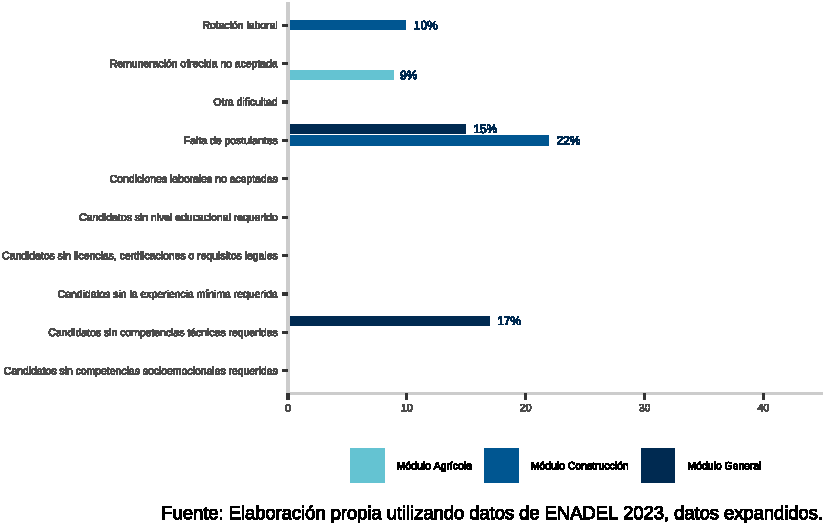
\includegraphics[width=1\textwidth,height=\textheight]{Reporte_files/figure-pdf/fig-dificultad-1.pdf}

}

\end{figure}%

\newpage

\subsubsection{Educación y
experiencia}\label{educaciuxf3n-y-experiencia}

El 86,5\% de los cargos\footnote{Esta pregunta sólo se realiza para las
  ocupaciones señaladas en el módulo de ``Otros Cargos''.} consultados
tienen algún requisito de nivel educacional. La
Figura~\ref{fig-educ-tot} muestra la frecuencia con la que se solicita
cada nivel educacional como requisito.

\begin{figure}[H]

\caption{\label{fig-educ-tot}Frecuencia de requisitos educacionales
requeridos}

\centering{

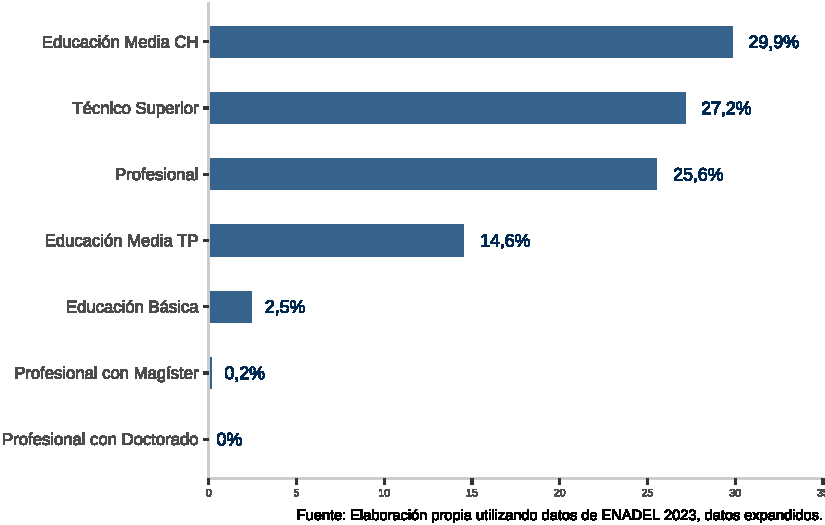
\includegraphics{Reporte_files/figure-pdf/fig-educ-tot-1.pdf}

}

\end{figure}%

Al consultar sobre experiencia requerida para el cargo, en el 33,8\% de
los casos se declara que el cargo no requiere experiencia. Para aquellas
ocupaciones donde si se señala experiencia laboral como uno de los
requisitos, el promedio total es de 2,6 años de experiencia (con un
error estándar de 0,12), sin haber mucha variación a través de los
distintos tamaños de empresa: se solicitan 2.8, 2.4 y 2.6 años en
promedio para empresas pequeñas, medianas y grandes, respectivamente.

\begin{table}

\caption{\label{tbl-exp_mean_sector}Experiencia laboral promedio
solicitada por sector de actividad económica.}

\centering{

\centering
\begin{tabular}{>{\raggedright\arraybackslash}p{9cm}>{\raggedright\arraybackslash}p{3cm}>{\raggedleft\arraybackslash}p{3cm}}
\toprule
Sector de Actividad Económica & \% que solicita experiencia & Experiencia promedio (años)\\
\midrule
Actividades financieras y de seguros & 78,6\% & 2,6\\
Transporte y almacenamiento & 74,4\% & 2,5\\
Información y comunicaciones & 72,8\% & 2,3\\
Actividades profesionales & 72\% & 3,4\\
Industria manufacturera & 70,1\% & 2,6\\
\addlinespace
Servicios administrativos y de apoyo & 68,7\% & 2,3\\
Actividades inmobiliarias & 68,4\% & 2,1\\
Construcción & 62,6\% & 3,0\\
Comercio & 59,8\% & 2,2\\
Silvoagropecuario & 59,3\% & 2,2\\
\addlinespace
Pesca y acuicultura & 55,8\% & 1,9\\
Administración pública & 55,1\% & 2,6\\
Alojamiento y de servicio de comidas & 54,3\% & 1,9\\
\bottomrule
\multicolumn{3}{l}{\rule{0pt}{1em}Fuente: Elaboración propia utilizando datos de ENADEL 2023, datos expandidos.}\\
\end{tabular}

}

\end{table}%

La Figura~\ref{fig-top_and_bottom} muestra a los tres sectores con mayor
y menor proporción de empresas que tienen requisitos de experiencia para
las nuevas contrataciones en los cargos consultados. Para aquellos
sectores que solicitan experiencia con más frecuencia, el promedio
supera los dos años, siendo ``Actividades financieras y de seguros'' el
sector que más solicita, con 2.6 años en promedio.

\begin{figure}[H]

\caption{\label{fig-top_and_bottom}Años de experiencia promedio para
sectores que solicitan más y menos experiencia}

\centering{

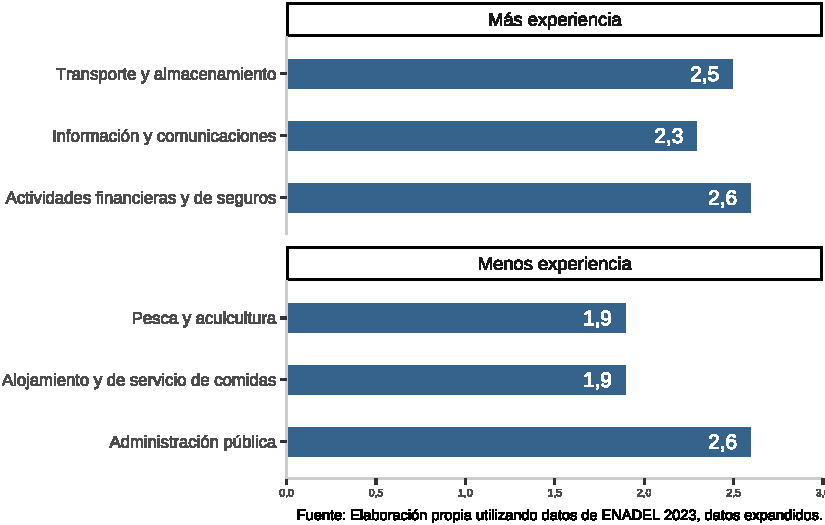
\includegraphics{Reporte_files/figure-pdf/fig-top_and_bottom-1.pdf}

}

\end{figure}%

Con respecto a la experiencia solicitada por sector de actividad
económica, los sectores de ``Pesca y acuicultura'' y de ``Alojamiento y
de servicio de comidas'' son los que requieren menos años de experiencia
(\text{1,9} años en promedio); mientras que ``Actividades
profesionales'' es el que más años de experiencia requiere, con
\text{3,4} años en promedio.

\subsubsection{Canales de reclutamiento}\label{canales-de-reclutamiento}

Frente a la pregunta \footnote{Esta pregunta sólo se realiza para las
  ocupaciones señaladas en el módulo de ``Otros Cargos''.}:

\emph{¿Nos puede indicar que canales o medios de contratación utilizó en
los procesos de reclutamiento y búsqueda de personas?}

La Tabla 18 muestra la proporción de cada uno de los canales
mencionados, tanto para el primer canal mencionado, como para el total.

\begin{table}

\caption{\label{tbl-canal}Canales de reclutamiento más utilizados,
ENADEL 2023}

\centering{

\centering
\begin{tabular}{>{\raggedright\arraybackslash}p{9cm}>{\raggedright\arraybackslash}p{3cm}>{\raggedright\arraybackslash}p{3cm}}
\toprule
Canal de reclutamiento & 1° Canal & Total\\
\midrule
Recomendaciones de trabajadores de la empresa u otros actores & 21\% & 21,3\%\\
Plataforma web de empleo pagada & 28,2\% & 20,2\%\\
Redes sociales & 13,3\% & 13,2\%\\
Redes personales del empleador & 8,8\% & 10,8\%\\
Plataforma web de empleo privada gratuita & 7\% & 8,6\%\\
\addlinespace
Oficina Municipal de Información Laboral & 5,8\% & 6,8\%\\
Avisos en la calle o banco de Curriculums & 2,6\% & 3,9\%\\
Diario o radio & 4\% & 3,6\%\\
Contratación de empresas de reclutamiento & 4,3\% & 3,5\%\\
Bolsa Nacional de Empleo & 2\% & 3\%\\
\addlinespace
Otro & 1,7\% & 2,8\%\\
Redes de profesionales, egresados o contacto con universidades & 1,3\% & 2,2\%\\
\bottomrule
\multicolumn{3}{l}{\rule{0pt}{1em}Fuente: Elaboración propia utilizando datos de ENADEL 2023, datos expandidos.}\\
\end{tabular}

}

\end{table}%

Considerando el total de respuestas (los tres canales mencionados), se
tiene que las principales vías de reclutamiento son ``Recomendaciones de
trabajadores de la empresa u otros actores'' con 21,3\% y ``Plataforma
web de empleo pagada'' con un 20,2\%. Los canales menos utilizados según
las menciones son, ``Redes de profesionales, egresados o contacto con
universidades'' con apenas un 2,2\%, y ``Bolsa Nacional de Empleo'', con
el 3\% .

\subsubsection{Conocimiento de instituciones y
programas}\label{conocimiento-de-instituciones-y-programas}

Frente a la pregunta: \emph{¿Conoce, y ha accedido a beneficios de las
siguientes instituciones o servicios públicos?}

SENCE SENCE se posiciona como la institución y/o servicio con más
conocimiento, con un 94,2\% de conocimiento, seguido de CORFO (85,6\%) y
OMIL (75,9\%). SENCE lidera el ranking de uso, con un 40,2\%, seguido
por las OMIL (34\%) y la BNE (17,4\%). Chile Valora es la institución
con menor conocimiento, con sólo un 36\% de los encuestados declarando
que lo conocen.

\begin{figure}[H]

\caption{\label{fig-conocimiento_1}Conocimiento sobre beneficios de
instituciones o servicios públicos, ENADEL 2023.}

\centering{

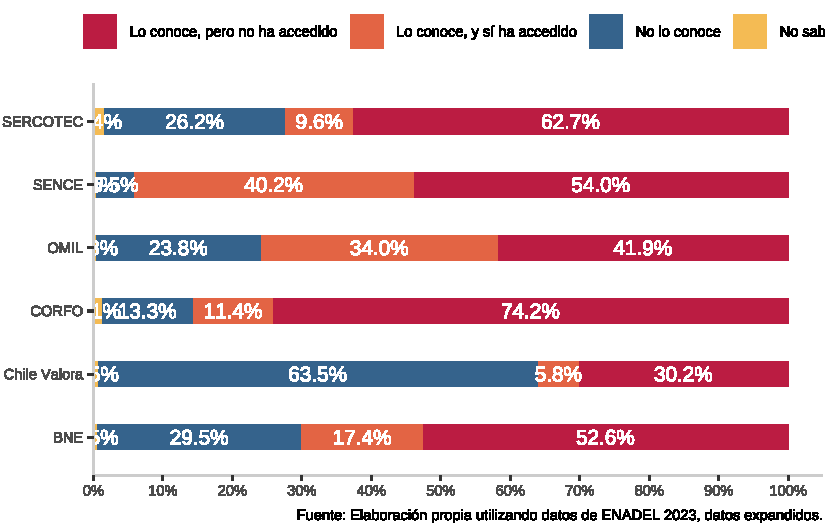
\includegraphics{Reporte_files/figure-pdf/fig-conocimiento_1-1.pdf}

}

\end{figure}%

\begin{verbatim}
[1] "despega"  "sej"      "btm"      "expmayor" "aprendiz" "ft"       "ferias"  
[8] "digpyme"  "fosis"   
\end{verbatim}

Por otro lado, la frente a la pregunta: \emph{¿Conoce, y ha accedido a
beneficios de los siguientes programas o subsidios públicos?}

Los subsidios Subsidio al Empleo Joveny Bono Trabajo Mujer son los
programas con un mayor nivel de conocimiento (75,6\%y 69,9\%,
respectivamente), seguido por el programa FOSIS (57,5\%) y las FERIAS
LABORALES (56,7\%). Con respecto al nivel de uso, los programas de
subsidio también lideran, seguido de la FRANQUICIA TRIBUTARIA ( 24,2\%).

\begin{figure}[H]

\caption{\label{fig-conocimiento_2}Conocimiento sobre beneficios de
programas o subsidios públicos, ENADEL 2023.}

\centering{

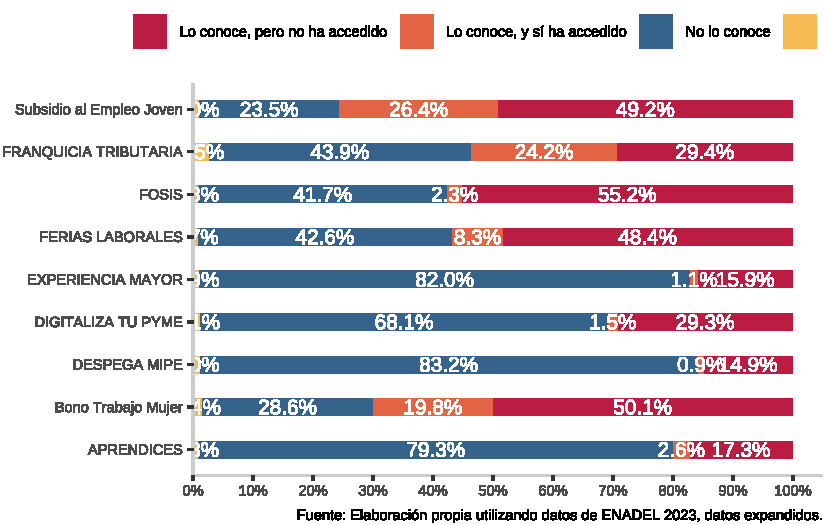
\includegraphics{Reporte_files/figure-pdf/fig-conocimiento_2-1.pdf}

}

\end{figure}%

La mayoría de los programas tienen un bajo nivel de conocimiento:
DESPEGA MIPE, EXPERIENCIA MAYOR y APRENDICES tienen tasas de
conocimiento inferiores al 19,9\%, y DIGITALIZA TU PYME de alrededor del
30,8\%.

\subsubsection{Apéndice A: Ocupaciones de Difícil
Cobertura}\label{apuxe9ndice-a-ocupaciones-de-difuxedcil-cobertura}

\begin{table}

\caption{\label{tbl-vacantes_totales}}

\centering{

\centering
\begin{tabular}{>{\raggedright\arraybackslash}p{9cm}>{\raggedleft\arraybackslash}p{3cm}>{\raggedright\arraybackslash}p{3cm}}
\toprule
Glosa & Vacantes & CV\\
\midrule
Obreros de explotaciones agrícolas & 15063 & 57,8\%\\
Especialistas en políticas y servicios de personal & 2459 & 25\%\\
Obreros de carga & 2192 & 37,9\%\\
Soldadores y oxicortadores & 2084 & 73,4\%\\
Empacadores manuales & 1887 & 70,6\%\\
\addlinespace
Gásfiter e instaladores de tuberías & 1742 & 74,5\%\\
Auxiliares de aseo de oficinas, hoteles y otros establecimientos & 1706 & 45,5\%\\
Guardias de seguridad & 1614 & 50,2\%\\
Técnicos en electricidad & 1521 & 70,4\%\\
Conductores de automóviles, taxis y camionetas & 1485 & 64,6\%\\
\addlinespace
Empleados encargados del control de abastecimiento e inventario & 1442 & 76\%\\
Ayudantes de cocina & 1251 & 69\%\\
Especialistas y asesores de gestión & 1187 & 100\%\\
Vendedores y asistentes de venta de tiendas, almacenes y puestos de mercado & 1030 & 60\%\\
Obreros de la industria manufacturera no clasificados previamente & 969 & 62,4\%\\
\addlinespace
Conductores de camiones pesados y de alto tonelaje & 904 & 62,7\%\\
Carpinteros de obra & 844 & 60,3\%\\
Obreros de explotaciones ganaderas & 811 & 23,5\%\\
Mensajeros, estafetas, maleteros y repartidores de folletos y diarios a domicilio & 725 & 39,9\%\\
Cocineros & 703 & 56,2\%\\
\addlinespace
Auxiliares de mantenimiento (pequeñas reparaciones) & 678 & 39,8\%\\
Profesionales de ventas técnicas y médicas (excluyendo las TIC) & 662 & 75\%\\
Garzones de mesa & 622 & 42,5\%\\
Electricistas de obras & 618 & 20,5\%\\
Cocineros de comida rápida & 593 & 61,5\%\\
\addlinespace
Catadores, clasificadores y controladores de calidad de alimentos y bebidas & 530 & 43,6\%\\
Limpiadores de vehículos & 510 & 68,3\%\\
Mecánicos y ajustadores electricistas & 499 & 36\%\\
Mecánicos y reparadores de máquinas agrícolas e industriales & 499 & 52,7\%\\
Directores, gerentes y administradores de comercialización & 492 & 72,2\%\\
\addlinespace
Desarrolladores de software & 470 & 66,7\%\\
Mecánicos de instalaciones de refrigeración y aire acondicionado & 466 & 45,4\%\\
Obreros de la construcción de edificios & 459 & 50,7\%\\
Técnicos y auxiliares paramédicos de enfermería & 450 & 40\%\\
Enfermeros profesionales & 433 & 20\%\\
\addlinespace
Ingenieros electrónicos & 433 & 20\%\\
Vendedores por internet y otros medios de comunicación & 413 & 25\%\\
Inspectores de la salud y técnicos en prevención de riesgos & 398 & 48\%\\
Agricultores y trabajadores calificados de cultivos extensivos & 391 & 27,9\%\\
Operadores de autoelevadoras y montacargas & 391 & 62,8\%\\
\addlinespace
Conductores de buses y trolebuses & 385 & 80,6\%\\
Operadores de grúas y aparatos elevadores & 375 & 58,9\%\\
Trabajadores de tareas administrativas generales & 364 & 69,9\%\\
Programadores de aplicaciones & 363 & 23,7\%\\
Directores, gerentes y administradores de empresas de construcción & 361 & 57,9\%\\
\addlinespace
Promotores de tiendas & 357 & 33,3\%\\
Operadores de máquinas para fabricar productos de papel & 353 & 50\%\\
Operadores de máquinas para fabricar productos de material plástico & 351 & 42,8\%\\
Mecánicos y reparadores de vehículos de motor & 341 & 48,1\%\\
Instaladores y reparadores en tecnología de la información y las comunicaciones & 338 & 51,9\%\\
\addlinespace
Representantes comerciales (excepto venta de productos y servicios industriales, farmacéuticos y de tecnologías de la información y las comunicaciones) & 316 & 44,2\%\\
Técnicos en electrónica & 304 & 83,3\%\\
Secretarios generales & 292 & 79\%\\
Empleados de informaciones, reclamos o sugerencias & 284 & 40\%\\
Vendedores de comidas al mostrador & 284 & 51,8\%\\
\addlinespace
Recepcionistas (funciones generales) & 253 & 36,9\%\\
Ayudantes de jardinería y horticultura & 225 & 15,7\%\\
Técnicos en asistencia al usuario de tecnología de la información y las comunicaciones & 216 & 25\%\\
Técnicos y asistentes en contabilidad & 191 & 53\%\\
Albañiles & 185 & 34,7\%\\
\addlinespace
Vendedores de entradas (entretenciones y eventos deportivos) y cajeros de comercio & 180 & 78,7\%\\
Ingenieros en telecomunicaciones & 175 & 50\%\\
Productores y trabajadores calificados de explotaciones agropecuarias mixtas & 161 & 72,4\%\\
Reguladores y operarios de máquinas herramientas & 151 & 63,2\%\\
Panaderos, pasteleros y confiteros & 147 & 51,6\%\\
\addlinespace
Otro personal de los servicios de protección no clasificados previamente & 146 & 25\%\\
Ejecutivos de préstamos y créditos & 144 & 29,4\%\\
Otros operarios de la construcción (obra gruesa) no clasificados previamente & 133 & 42,8\%\\
Buzos & 132 & 17,9\%\\
Clasificadores, probadores de productos e inspectores de calidad (excluyendo alimentos y bebidas) & 129 & 28,2\%\\
\addlinespace
Químicos farmacéuticos & 129 & 57,3\%\\
Directores, gerentes y administradores de restaurantes & 127 & 17\%\\
Mecánicos y reparadores en electrónica & 126 & 66,7\%\\
Reponedores de estanterías & 125 & 35,9\%\\
Agentes responsables de adquisiciones & 119 & 38,4\%\\
\addlinespace
Contadores & 118 & 33\%\\
Técnicos de radiodifusión y grabación audiovisual & 117 & 25\%\\
Directores, gerentes y administradores de servicios de tecnología de la información y las comunicaciones & 115 & 66,2\%\\
Supervisores de locales comerciales, tiendas y almacenes & 114 & 19,6\%\\
Abogados & 111 & 40\%\\
\addlinespace
Operadores de plantas y máquinas para fabricar productos químicos & 107 & 33,3\%\\
Técnicos en ingeniería mecánica & 105 & 47,8\%\\
Operadores de maquinaria agrícola y forestal móvil & 102 & 68,2\%\\
Fumigadores y otros controladores de plagas y malezas & 97 & 48,5\%\\
Ingenieros en prevención de riesgos y otros profesionales de la seguridad e higiene laboral y ambiental & 95 & 45,6\%\\
\addlinespace
Técnicos agropecuarios (incluyendo acuícolas) & 94 & 75\%\\
Bomberos de gasolineras & 92 & 75\%\\
Analistas de sistemas & 91 & 59,4\%\\
Obreros de explotaciones agropecuarias & 90 & 39,9\%\\
Desarrolladores Web y multimedia & 83 & 33,3\%\\
\addlinespace
Ingenieros civiles, ingenieros en construcción y constructores civiles & 83 & 69,9\%\\
Otros desarrolladores y analistas de software y multimedia no clasificados previamente & 83 & 33,3\%\\
Instaladores y reparadores de líneas eléctricas & 82 & 66,7\%\\
Operadores de máquinas de movimiento de tierras & 79 & 58,8\%\\
Profesores de educación básica & 73 & 33,3\%\\
\addlinespace
Directores, gerentes y administradores de comercios al por mayor y al por menor & 71 & 14,9\%\\
Técnicos en ciencias físicas y químicas & 71 & 40\%\\
Operadores de máquinas de embalaje, embotellamiento y etiquetado & 70 & 50\%\\
Ingenieros químicos & 68 & 50\%\\
Carniceros y pescaderos & 67 & 43,9\%\\
\addlinespace
Otros especialistas en bases de datos y en redes de computadores no clasificados previamente & 65 & 66,7\%\\
Revisores y cobradores de los transportes públicos & 65 & 25\%\\
Profesionales de la publicidad y la comercialización & 60 & 40\%\\
Operadores de instalaciones de procesamiento de la madera & 59 & 41,7\%\\
Recolectores de basura y material reciclable & 59 & 25\%\\
\addlinespace
Veterinarios & 58 & 45,9\%\\
Supervisores de la construcción & 57 & 9,6\%\\
Cartógrafos y agrimensores & 54 & 50\%\\
Directores, gerentes y administradores de industrias manufactureras & 51 & 92,8\%\\
Operadores de máquinas para elaborar alimentos, bebidas y cigarrillos & 46 & 71,7\%\\
\addlinespace
Directores, gerentes y administradores de recursos humanos & 45 & 39,9\%\\
Recepcionistas de hoteles & 42 & 50,3\%\\
Técnicos de ingeniería de las telecomunicaciones & 42 & 50\%\\
Secretarios administrativos y ejecutivos & 41 & 48,1\%\\
Digitadores de datos & 39 & 50\%\\
\addlinespace
Profesionales de ventas de tecnología de la información y las comunicaciones (TIC) & 38 & 25\%\\
Directores, gerentes y administradores de producción y operaciones agropecuarias y de silvicultura & 37 & 75\%\\
Técnicos en construcción y topógrafos & 37 & 60\%\\
Conductores de motocicletas & 36 & 50\%\\
Ingenieros mecánicos & 35 & 93,5\%\\
\addlinespace
Montadores de estructuras metálicas & 35 & 43,4\%\\
Otras ocupaciones elementales no clasificadas previamente & 35 & 23,9\%\\
Técnicos y asistentes veterinarios & 34 & 43,4\%\\
Administradores de sistemas & 33 & 31,6\%\\
Empleados y asistentes de recursos humanos & 32 & 32,8\%\\
\addlinespace
Operadores de máquinas de preparación de fibras, hilado y devanado & 32 & 100\%\\
Instaladores de parqué, cerámicas, baldosas y alfombras & 31 & 25,4\%\\
Operadores de instalaciones de producción de energía & 31 & 100\%\\
Constructores de casas & 30 & 62\%\\
Directores, gerentes y administradores de finanzas & 30 & 14,7\%\\
\addlinespace
Tripulantes de cubierta de barco & 30 & 46,5\%\\
Autores y otros escritores & 28 & 50\%\\
Bármanes & 28 & 50,8\%\\
Diseñadores de productos y de vestuario & 28 & 88,9\%\\
Técnicos forestales & 28 & 50\%\\
\addlinespace
Agentes de aduana & 27 & 27,7\%\\
Obreros forestales & 27 & 25\%\\
Trabajadores de explotaciones de acuicultura & 27 & 69,6\%\\
Barnizadores y pulverizadores de productos manufacturados & 26 & 50\%\\
Impresores & 26 & 41,7\%\\
\addlinespace
Representantes de ventas de puerta a puerta (venta a hogares) & 26 & 50\%\\
Obreros de pesca y acuicultura & 24 & 25\%\\
Operadores de instalaciones de vidriería y cerámica & 24 & 50\%\\
Otros técnicos en actividades culturales y artísticas no clasificados previamente & 23 & 100\%\\
Ingenieros industriales y de producción & 22 & 68\%\\
\addlinespace
Instaladores o reparadores de techos & 22 & 100\%\\
Directores, gerentes y administradores de empresas de abastecimiento, almacenamiento y distribución & 21 & 40\%\\
Agricultores y trabajadores calificados de plantaciones de árboles y arbustos & 20 & 75\%\\
Diseñadores gráficos y de multimedia & 20 & 34,2\%\\
Ebanistas y mueblistas & 18 & 50\%\\
\addlinespace
Chefs & 17 & 99,4\%\\
Empleados encargados de las nóminas o registros de remuneraciones & 17 & 37,6\%\\
Operadores y reguladores de máquinas para trabajar la madera & 17 & 66,7\%\\
Personal de pompas fúnebres y embalsamadores & 17 & 100\%\\
Agricultores y trabajadores calificados de huertas, invernaderos, viveros y jardines & 15 & 25\%\\
\addlinespace
Empleados de centros de llamadas de informaciones & 15 & 20\%\\
Técnicos en redes y sistemas de computadores & 15 & 20\%\\
Empleados de servicios de transporte & 14 & 61,4\%\\
Profesionales de las relaciones públicas & 14 & 80\%\\
Directores, gerentes y administradores de hoteles & 13 & 33,3\%\\
\addlinespace
Ensambladores no clasificados previamente & 13 & 50\%\\
Trabajadores ambulantes de servicios & 13 & 33,3\%\\
Analistas financieros & 12 & 33,3\%\\
Profesionales del trabajo social & 12 & 15,6\%\\
Supervisores de oficina & 12 & 25\%\\
\addlinespace
Agrónomos y profesionales del ámbito forestal y pesquero & 11 & 25\%\\
Dinamiteros y pegadores & 10 & 50\%\\
Maquinistas de locomotoras & 10 & 100\%\\
Otros ingenieros no clasificados previamente & 10 & 25\%\\
Limpiadores de ventanas & 8 & 100\%\\
\addlinespace
Personal directivo de la administración pública & 8 & 72,4\%\\
Biólogos, botánicos, zoólogos, genetistas y farmacólogos & 7 & 20\%\\
Delineantes y dibujantes técnicos & 7 & 33,3\%\\
Psicólogos & 7 & 20\%\\
Terapeutas ocupacionales & 7 & 33,3\%\\
\addlinespace
Técnicos de los servicios jurídicos & 7 & 25\%\\
Técnicos en trabajo social & 7 & 100\%\\
Cuidadores de animales & 6 & 33,3\%\\
Auxiliares y ayudantes de registros de contabilidad y cálculo de costos & 5 & 60\%\\
Capitanes y oficiales de cubierta & 5 & 25,3\%\\
\addlinespace
Ingenieros eléctricos & 5 & 25\%\\
Ingenieros medioambientales & 5 & 18,4\%\\
Médicos generales & 5 & 100\%\\
Operarios en cemento armado & 5 & 33,3\%\\
Otros vendedores no clasificados previamente & 5 & 33,3\%\\
\addlinespace
Periodistas & 5 & 20\%\\
Bomberos & 4 & 33,3\%\\
Directores y gerentes generales de empresas & 4 & 40\%\\
Operadores de máquinas de lavanderías & 4 & 50\%\\
Agentes inmobiliarios & 3 & 33,4\%\\
\addlinespace
Lavanderos y planchadores manuales & 3 & 25\%\\
Técnicos de la Web & 3 & 25\%\\
Urbanistas e ingenieros de transporte y tránsito & 3 & 33,3\%\\
Clasificadores de desechos & 2 & 50\%\\
Empleados administrativos de archivos & 2 & 33,3\%\\
\addlinespace
Costureros y bordadores & 1 & 50\%\\
Directores, gerentes y administradores de servicios de bienestar social & 1 & 100\%\\
Agentes de empleo y contratistas de personal & 0 & NaN\%\\
Agentes de la administración pública para la aplicación de la ley no clasificados previamente & 0 & NaN\%\\
Agentes de la administración tributaria & 0 & NaN\%\\
\addlinespace
Agentes de seguros y ejecutivos de fondos de pensiones & 0 & NaN\%\\
Agentes de servicios de tramitación y entrega de licencias y permisos & 0 & NaN\%\\
Agricultores y trabajadores calificados de cultivos mixtos & 0 & NaN\%\\
Amas de llaves, mayordomos domésticos y dueños/administradores de pequeños establecimientos de alojamiento & 0 & NaN\%\\
Aparejadores y empalmadores de cables no eléctricos & 0 & NaN\%\\
\addlinespace
Arquitectos & 0 & NaN\%\\
Artesanos de los tejidos, el cuero y materiales similares & 0 & NaN\%\\
Asesores financieros y en inversiones & 0 & NaN\%\\
Asistentes de aula e inspectores de patio & 0 & NaN\%\\
Auxiliares de servicio a bordo de aeronaves y barcos & 0 & NaN\%\\
\addlinespace
Auxiliares y ayudantes de servicios estadísticos, financieros y de seguros & 0 & NaN\%\\
Ayudantes de ambulancia & 0 & NaN\%\\
Barrenderos & 0 & NaN\%\\
Bioquímicos & 0 & NaN\%\\
Cajeros de bancos y de oficinas de correo & 0 & NaN\%\\
\addlinespace
Carteros y empleados de servicios de correos y encomiendas & 0 & NaN\%\\
Chapistas y caldereros & 0 & NaN\%\\
Cobradores & 0 & NaN\%\\
Conductores de vehículos y máquinas de tracción animal & 0 & NaN\%\\
Conserjes & 0 & NaN\%\\
\addlinespace
Controladores de instalaciones de procesamiento de productos químicos & 0 & NaN\%\\
Controladores de procesos de producción de metales & 0 & NaN\%\\
Corredores comerciales y consignatarios & 0 & NaN\%\\
Cosmetólogos y especialistas en tratamientos de belleza & 0 & NaN\%\\
Criadores de ganado & 0 & NaN\%\\
\addlinespace
Cristaleros & 0 & NaN\%\\
Cuidadores de niños en instituciones y a domicilios & 0 & NaN\%\\
Dentistas & 0 & NaN\%\\
Dietistas y nutricionistas & 0 & NaN\%\\
Directores de cine, radio y teatro & 0 & NaN\%\\
\addlinespace
Directores, gerentes y administradores de centros deportivos, de esparcimiento y culturales & 0 & NaN\%\\
Directores, gerentes y administradores de explotaciones mineras & 0 & NaN\%\\
Directores, gerentes y administradores de investigación y desarrollo & 0 & NaN\%\\
Directores, gerentes y administradores de otros servicios no clasificados previamente & 0 & NaN\%\\
Directores, gerentes y administradores de políticas empresariales y planificación & 0 & NaN\%\\
\addlinespace
Directores, gerentes y administradores de producción y operaciones de acuicultura y pesca & 0 & NaN\%\\
Directores, gerentes y administradores de publicidad y relaciones públicas & 0 & NaN\%\\
Directores, gerentes y administradores de servicios de cuidados infantiles & 0 & NaN\%\\
Directores, gerentes y administradores de servicios de educación & 0 & NaN\%\\
Directores, gerentes y administradores de servicios de salud & 0 & NaN\%\\
\addlinespace
Directores, gerentes y administradores de servicios financieros & 0 & NaN\%\\
Dirigentes de organizaciones sociales y/o políticas (sindicatos, organizaciones sociales, partidos políticos, entre otras) & 0 & NaN\%\\
Diseñadores y administradores de bases de datos & 0 & NaN\%\\
Diseñadores y decoradores de interior & 0 & NaN\%\\
Economistas & 0 & NaN\%\\
\addlinespace
Educadores de párvulos & 0 & NaN\%\\
Empleados de agencias de viajes & 0 & NaN\%\\
Empleados de cálculo de los insumos y materiales para la producción & 0 & NaN\%\\
Encuadernadores & 0 & NaN\%\\
Ensambladores de equipos eléctricos y electrónicos & 0 & NaN\%\\
\addlinespace
Ensambladores de maquinaria mecánica & 0 & NaN\%\\
Especialistas en formación del personal & 0 & NaN\%\\
Especialistas en métodos pedagógicos & 0 & NaN\%\\
Especialistas en políticas de administración & 0 & NaN\%\\
Filósofos, historiadores y especialistas en ciencias políticas & 0 & NaN\%\\
\addlinespace
Geólogos y geofísicos & 0 & NaN\%\\
Guías de turismo & 0 & NaN\%\\
Herramentistas & 0 & NaN\%\\
Herreros y forjadores & 0 & NaN\%\\
Ingenieros biomédicos & 0 & NaN\%\\
\addlinespace
Ingenieros en minas y metalúrgicos & 0 & NaN\%\\
Inspectores de aduana & 0 & NaN\%\\
Instaladores de material aislante y de insonorización & 0 & NaN\%\\
Instructores de acondicionamiento físico y actividades recreativas & 0 & NaN\%\\
Joyeros, orfebres y plateros & 0 & NaN\%\\
\addlinespace
Kinesiólogos & 0 & NaN\%\\
Laboratoristas dentales o técnicos en prótesis dentales & 0 & NaN\%\\
Limpiadores de fachadas y deshollinadores & 0 & NaN\%\\
Locutores de radio, televisión y otros medios de comunicación & 0 & NaN\%\\
Mecánicos y reparadores de motores de avión & 0 & NaN\%\\
\addlinespace
Miembros del poder ejecutivo y legislativo & 0 & NaN\%\\
Moldeadores y macheros & 0 & NaN\%\\
Médicos especialistas & 0 & NaN\%\\
Músicos, cantantes y compositores & 0 & NaN\%\\
Obreros de la minería & 0 & NaN\%\\
\addlinespace
Obreros de obras públicas & 0 & NaN\%\\
Oficiales maquinistas en navegación & 0 & NaN\%\\
Operadores de incineradores y de instalaciones de tratamiento de agua & 0 & NaN\%\\
Operadores de instalaciones de procesamiento de metales & 0 & NaN\%\\
Operadores de instalaciones de procesamiento de minerales y rocas & 0 & NaN\%\\
\addlinespace
Operadores de máquinas de acabado de metales (pulidores, galvanizadores y recubridores de metales) & 0 & NaN\%\\
Operadores de máquinas de coser & 0 & NaN\%\\
Operadores de máquinas de vapor y calderas & 0 & NaN\%\\
Operadores de máquinas para fabricar cemento y otros productos minerales & 0 & NaN\%\\
Operadores de máquinas para fabricar productos de caucho & 0 & NaN\%\\
\addlinespace
Operadores de máquinas para fabricar productos textiles y artículos de piel y cuero no clasificados previamente & 0 & NaN\%\\
Operadores de máquinas y de instalaciones fijas no clasificados previamente & 0 & NaN\%\\
Operadores de telares y otras máquinas tejedoras & 0 & NaN\%\\
Operarios de la conservación de frutas, legumbres y verduras & 0 & NaN\%\\
Operarios de la elaboración de productos lácteos & 0 & NaN\%\\
\addlinespace
Operarios del tratamiento de la madera & 0 & NaN\%\\
Organizadores de conferencias y eventos & 0 & NaN\%\\
Otro personal de apoyo administrativo no clasificado previamente & 0 & NaN\%\\
Otro personal de limpieza no clasificado previamente & 0 & NaN\%\\
Otros criadores y trabajadores calificados de la cría de animales no clasificados previamente & 0 & NaN\%\\
\addlinespace
Otros directores, gerentes y administradores de servicios administrativos no clasificados previamente & 0 & NaN\%\\
Otros empleados de servicios de información al cliente no clasificados previamente & 0 & NaN\%\\
Otros profesionales de la educación no clasificados previamente & 0 & NaN\%\\
Otros técnicos en ciencias físicas y en ingeniería no clasificados previamente & 0 & NaN\%\\
Patronistas y cortadores de telas & 0 & NaN\%\\
\addlinespace
Perforadores y sondistas de pozos & 0 & NaN\%\\
Pescadores de alta mar & 0 & NaN\%\\
Pescadores en agua dulce y en aguas costeras & 0 & NaN\%\\
Pilotos de aviación & 0 & NaN\%\\
Pintores de carteles, pintores decorativos y grabadores & 0 & NaN\%\\
\addlinespace
Pintores y empapeladores de paredes & 0 & NaN\%\\
Podólogos & 0 & NaN\%\\
Profesionales de la protección medioambiental & 0 & NaN\%\\
Profesionales de matronería & 0 & NaN\%\\
Profesionales en redes de computadores & 0 & NaN\%\\
\addlinespace
Profesores de educación media & 0 & NaN\%\\
Profesores de educación media técnico profesional (especialidades) y de formación laboral & 0 & NaN\%\\
Pulidores de metales y afiladores de herramientas & 0 & NaN\%\\
Químicos & 0 & NaN\%\\
Recolectores de dinero en máquinas expendedoras de venta automática y lectores de medidores & 0 & NaN\%\\
\addlinespace
Secretarios jurídicos & 0 & NaN\%\\
Secretarios médicos & 0 & NaN\%\\
Sociólogos, antropólogos, geógrafos y arqueólogos & 0 & NaN\%\\
Sopladores, modeladores, laminadores, cortadores y pulidores de vidrio & 0 & NaN\%\\
Supervisores de industrias manufactureras & 0 & NaN\%\\
\addlinespace
Supervisores de mantenimiento y limpieza en oficinas, hoteles y otros establecimientos & 0 & NaN\%\\
Supervisores de minas & 0 & NaN\%\\
Tapiceros & 0 & NaN\%\\
Tasadores & 0 & NaN\%\\
Tecnólogos médicos & 0 & NaN\%\\
\addlinespace
Telefonistas & 0 & NaN\%\\
Tipógrafos & 0 & NaN\%\\
Trabajadores agrícolas de subsistencia & 0 & NaN\%\\
Trabajadores calificados de la apicultura y la sericultura & 0 & NaN\%\\
Trabajadores de casa particular y asistentes domésticos & 0 & NaN\%\\
\addlinespace
Trabajadores de los cuidados personales en instituciones & 0 & NaN\%\\
Trabajadores forestales calificados & 0 & NaN\%\\
Tronzadores, labrantes y grabadores de piedra & 0 & NaN\%\\
Técnicos en ciencias biológicas (excluyendo la medicina) & 0 & NaN\%\\
Técnicos en control de procesos no clasificados previamente & 0 & NaN\%\\
\addlinespace
Técnicos en documentación sanitaria & 0 & NaN\%\\
Técnicos en educación parvularia & 0 & NaN\%\\
Técnicos en ingeniería de minas y metalurgia & 0 & NaN\%\\
Técnicos en operaciones de tecnología de la información y las comunicaciones & 0 & NaN\%\\
Técnicos en química industrial & 0 & NaN\%\\
\addlinespace
Técnicos y asistentes farmacéuticos & 0 & NaN\%\\
Técnicos y auxiliares paramédicos de alimentación & 0 & NaN\%\\
Técnicos ópticos y contactólogos & 0 & NaN\%\\
Yeseros, estucadores y revocadores & 0 & NaN\%\\
NA & 0 & NaN\%\\
\bottomrule
\multicolumn{3}{l}{\rule{0pt}{1em}Fuente: Elaboración propia utilizando datos de ENADEL 2023, datos expandidos.}\\
\end{tabular}

}

\end{table}%

\newpage
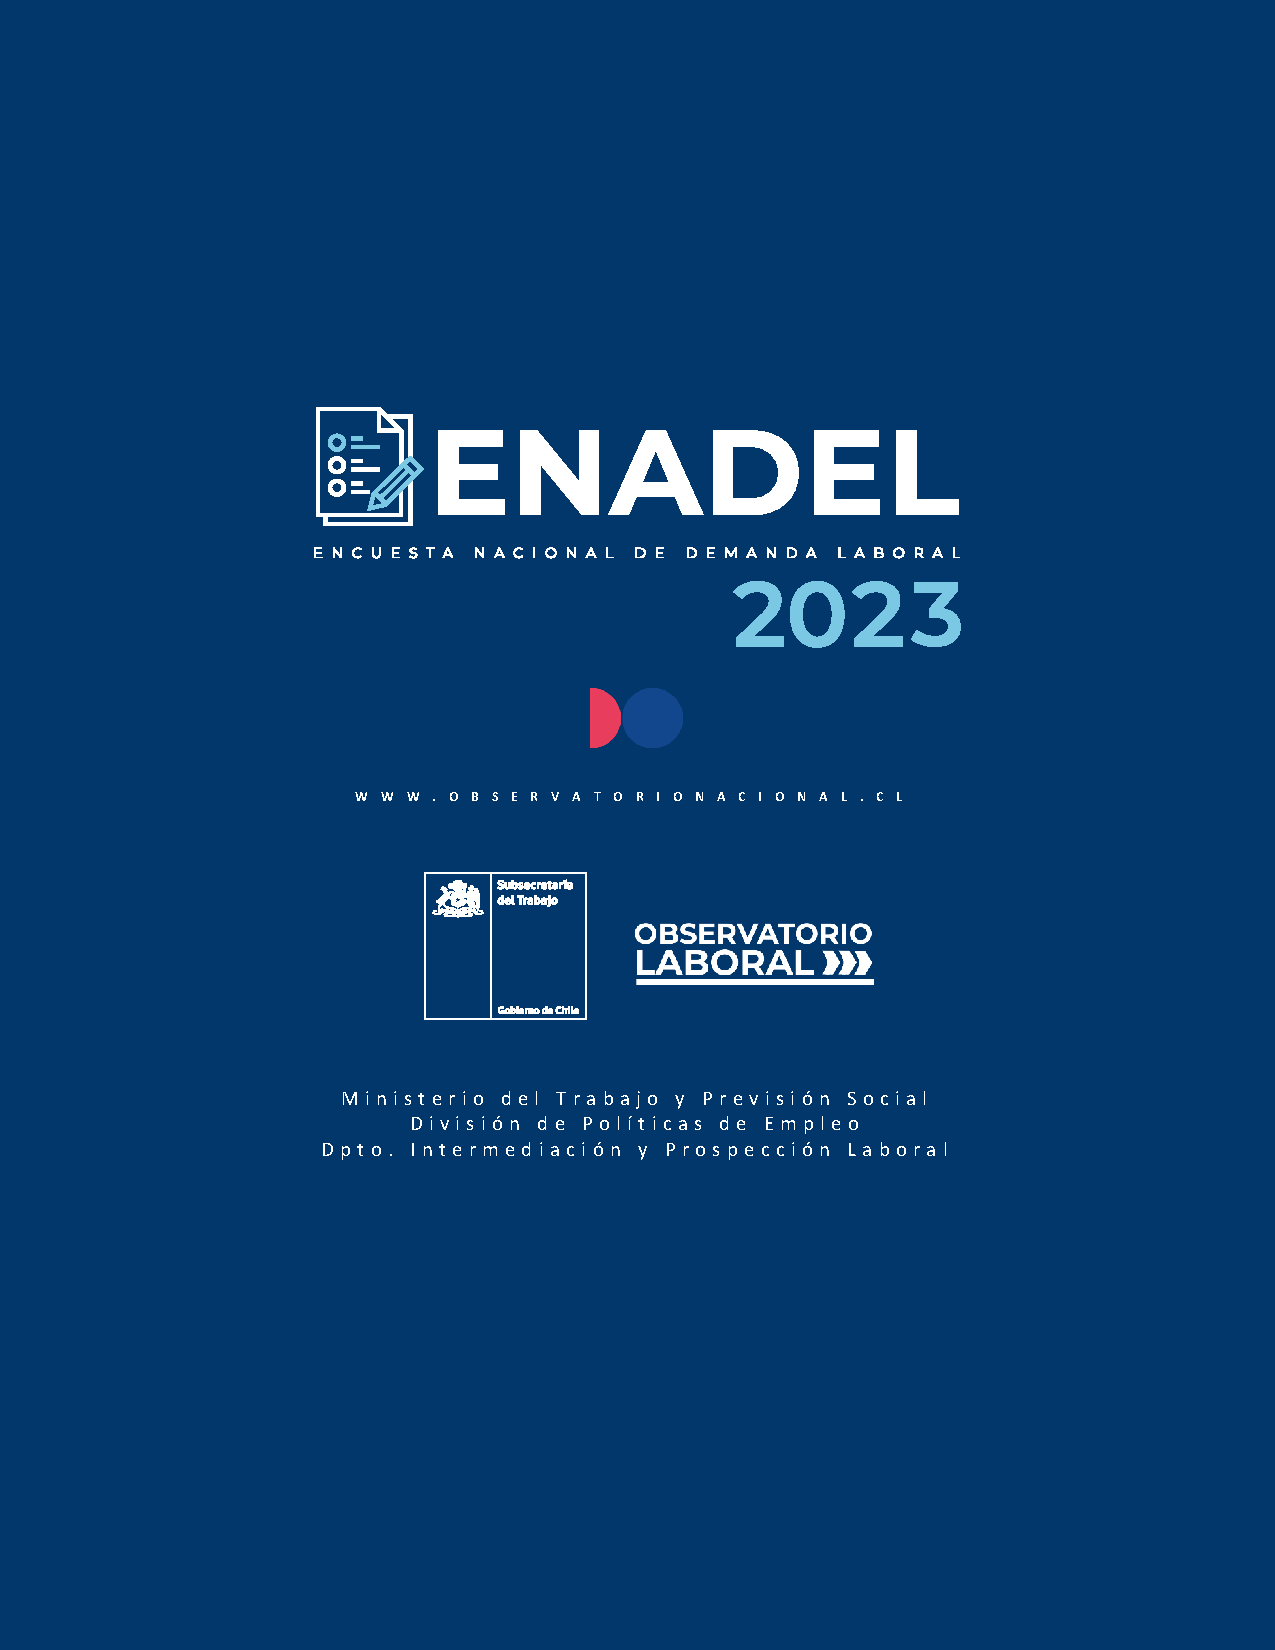
\includepdf[pages=-]{../Quarto/Portada/Portadas-Enadel-2023-5.pdf}




\end{document}
